\documentclass[table, 12pt]{article}
\usepackage[a4paper, top=25mm, bottom=25mm, left=20mm, right=20mm]{geometry}
\usepackage{graphicx}
\usepackage[T1]{fontenc}
\usepackage[default]{cantarell}
\usepackage{tocloft}
\usepackage{caption}
\usepackage{minted}
\usepackage{hyperref}
\usepackage{booktabs}
\usepackage{listings}
\usepackage{pdfpages}
\usepackage{pdflscape}
\usepackage{textpos}
\usepackage{scrhack}
\usepackage{xcolor}
\usepackage{mathptmx}
\usepackage{float}
\usepackage{longtable}
\usepackage{enumitem}
\usepackage{tasks}
\usepackage{tabularx}
\usepackage{titlesec}
\usepackage{graphicx}
\usepackage {float}

\newcommand{\red}{\color{red}}

\titleformat{\paragraph}
{\normalfont\normalsize\bfseries}{\theparagraph}{1em}{}
\titlespacing*{\paragraph}
{0pt}{3.95ex plus 1ex minus .2ex}{.5ex plus .2ex}

\begin{document}
\setlength{\parindent}{0em}

\begin{titlepage}
    \centering
    \vspace{2cm}
    \scshape\large Academic Year 2020/2021 \par
    \vfill
    
\includegraphics[width=200pt]{images/LogoPoliMI}\par\vspace{1cm}
    {\scshape\LARGE Computer Science and Engineering \par}
    \vspace{1.5cm}
    {\Large\bfseries System and Methods for Big and Unstructured Data \par}
    \vspace{0.5cm}
    {\huge\bfseries \textbf{Project Report - Neo4j} \par}
    \vspace{2cm}
    {\large{Matteo Falzi - 10638723\\ Fabio La Manna - 10620549 \\ Filippo Manzardo - 10864201 \\ Paolo Marzolo - 10668259 \\ Matteo Regge -  10619213}\par}
    \vfill
    {\large Prof. Marco Brambilla }
    \vfill
    {\large \textbf{}\\ \today \par}
\end{titlepage}
\hypersetup{%
    pdfborder = {0 0 0}
}
\thispagestyle{plain}
\pagenumbering{gobble}
\mbox{}

%%%%%%%%%%%%%%%%%%%%%%%%%%%%%%%%%%%%%%%%%%%%%%%%%%%%%%%%%%%%%%%%%

\section{Introduction}

The development of applications for tracing people contacts have seen an increasing interest due to Covid pandemic. The aim of these apps is to record paths and meetings of people in order to know their contacts and so to contain the spread of the virus. Recording paths means knowing where a person has been in the previous days, which places he visited and how much time he spent in there. This is important because in case of positive infection, these places can be advised in order to contact all the other people who were in the same place in the previous days. Recording meetings means knowing which people were directly in contact and how much time they spent together. This is helpful because in case of positive infection, all the people who were in contact with the infected can be found and then proceeded to be tested. The project consists of modelling a database to exploit these contact tracing applications using a NoSQL DB called Neo4J. 

\subsection{Delivery specification}
The goal of the project is: designing, storing and using a graph structure in a NoSQL DB for supporting a contact tracing application. The activities of the users can be: visiting some places or directed contacts. It has to be discerned the family group from the other people because family members are in contact by default. Every person must have some data: vaccines, tests and contagion information. In addition it has to be provided some queries and commands to retrieve information from the database. Obviously in order to do this, it will be needed a sample dataset that imitates a real Covid situation.

All the work done can be found at this link:
\href{https://github.com/pollomarzo/SAMBUD_proj}{GitHub Repo}

\subsection{Assumptions}

\begin{description}
\item[Users:] Users are over the age of 18. We have plenty of information about their addresses and birth. We have access to their Medical Records, tracking only information related to COVID, for example COVID Tests, COVID Vaccines, Health Status and general Health Risk. Due to the access of COVID Tests, we know if an user is Positive to the virus. The attribute "Last Confirm" indicates the date of the latest test in which the person could be resulted positive or negative. So the contagion date is implicit in this attribute because a person is revealed positive only when he obtains a positive result from the latest test. 
\item[Places:]The dataset containing places was retrieved from \href{http://download.geonames.org/export/dump/}{GeoNames} and it has been pre-processed for better use. We distinguish places that have rooms. To simplify, we assumed that every place exist and can be reached by an user. 
\item[Visits:] Every visit an user makes it's tracked by a third-party systems. We assume that in all the places, people are asked for their personal data and it is also registered the duration and the date of the visit.
\item[Contacts:]We consider a contact between the user and another person in a specific date and we always know the duration of the meeting. Every contact is mutual, meaning if P1 contacts P2, P2 contacts P1. The meeting between people can be tracked via the application on the smartphone but also on other devices like: bracers and smartwatches (we assume every person as at least a smartphone). 
\item[Personal data:]
We consider that a person may or may not have a vaccine/test. Also, we limit the vaccines into 4 categories: Pfizer, Astrazeneca, Johnson\&Johnson, Moderna. Any user cannot have more then one Vaccine/Test per day.
\item[Lives:] We consider family members as people who live in the same house. We modelled this with a relation "lives" between people who live in the same house.
\end{description} 
\newpage
%%%%%%%%%%%%%%%%%%%%%%%%%%%%%%%%%%%%%%%%%%%%%%%%%%%%%%%%%%%%%%%%%

\section{Relational Model}
To approach the problem, we developed an ER Model based of  3 main entities: Person, Medical Record and Place. 
Following the image of the ER diagram and the descriptions of the classes and relations.
\begin{figure}[H]
    \centering
    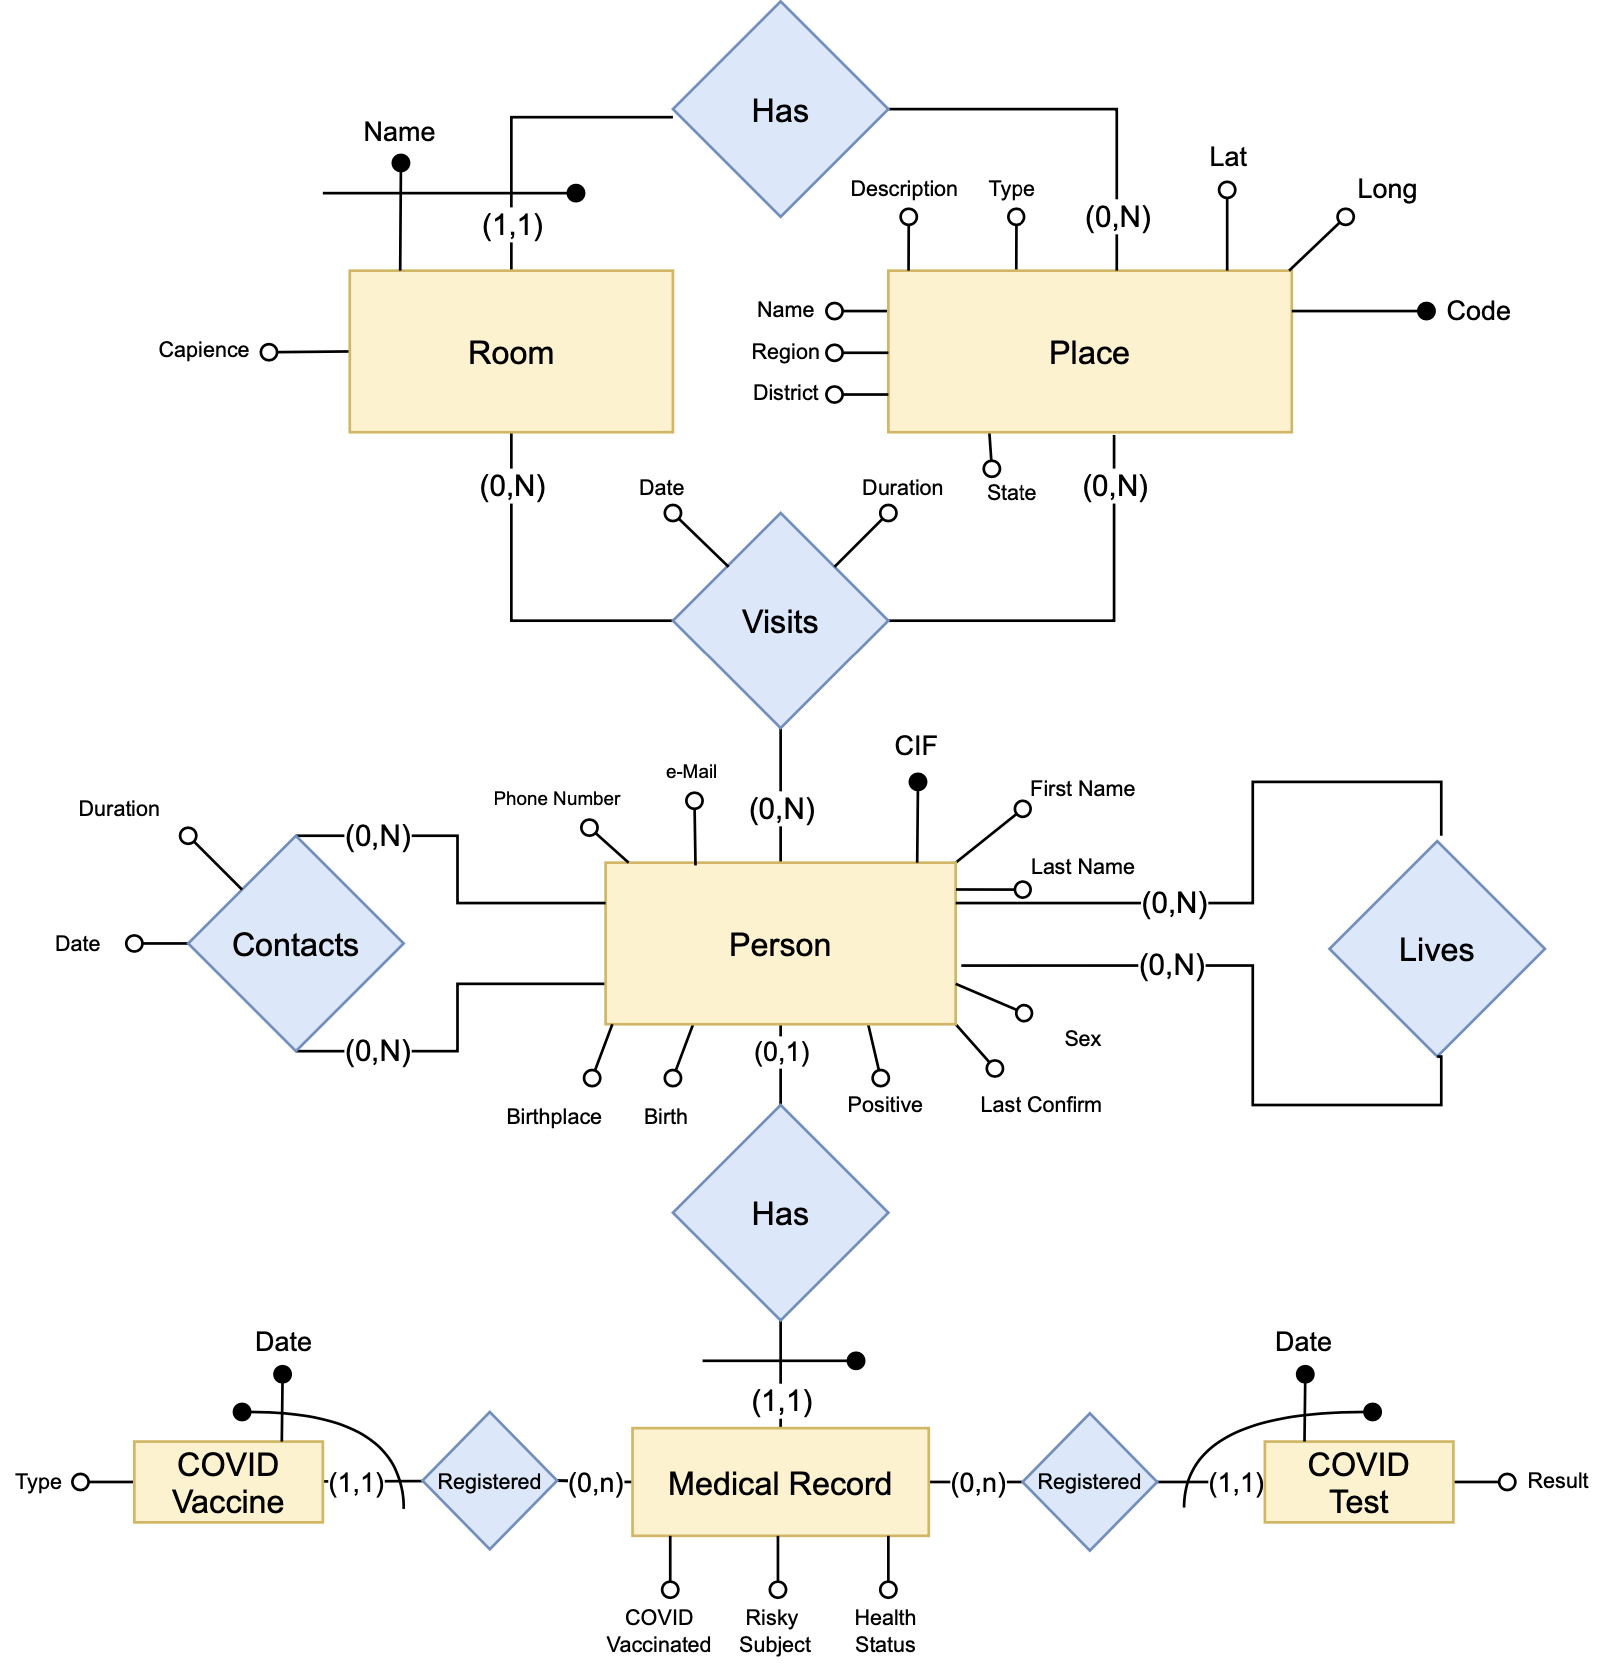
\includegraphics[width=\textwidth]{images/e.png}
    \caption{Entity-Relation Model}
    \label{fig:my_label}
\end{figure}
\subsection{Logical Model}
\begin{minted}
    [
    frame=lines,
    framesep=5mm,
    baselinestretch=1.5,
    escapeinside=||
    ]
    {python}
    ####### Entities #######
    Person(|\red{CIF}|,First_Name,Last_Name,Sex,Birth,Birthplace,Phone_Number,.. 
           ..e-Mail,Positive,Last_Confirm)
    Place(|\red{Code}|,Name,Lat,Long,CAP,State,Region,District,Type,Type_Desc)
    Rooms(|\red{Code}|,|\red{Name}|,Capience)
    Medical_Record(|\red{CIF}|,Covid_Vaccinated,Risky_Subject,Health_Status)
    Covid_Tests(|\red{CIF}|,|\red{Date}|,Results)
    Covid_Vaccines(|\red{CIF}|,|\red{Date}|,Type)
   
    ####### Relations #######
    Contacts(|\red{CIF}|,|\red{CIF}|,Date,Duration)
    Lives(|\red{CIF}|,|\red{CIF}|)
    Visits(|\red{CIF}|,|\red{Code}|,|\red{Name}|,Date,Duration)
    
            
\end{minted}

\section{Neo4j Implementation}
To generate entities and relations, we coded a python script called "generate\_dataset.py", in the latest DB there are:
\begin{itemize}
    \setlength\itemsep{-0.5em}
    \item ~$8000$ People  \\
    \item ~$30000$ Contacts \\
    \item ~$500$ Places \\
    \item ~$500$ Rooms \\
    \item ~$20000$ Visits  
\end{itemize}
For a total of $38904$ nodes and $88110$ relations.
These numbers can be modified through the variables found in the first lines of the script. \\
Once that the script has been executed, 9 output CSV files can be found in scripts/output. This file are later imported into Neo4j's database via some load queries listed in "scripts/load\_queries.txt".
\subsection{Queries}

Now we list some queries we wrote to inspect our database for useful information about COVID.

\subsubsection*{Query n. 1}
Find all the contacts a Positive Person made during the last 5 days, returning Names, Dates and Days Passed

\begin{minted}
    [
    frame=lines,
    framesep=5mm,
    baselinestretch=1.5,
    escapeinside=||
    ]
    {mysql}
MATCH (p1:Person)-|[|c:CONTACTS|]|-(p2:Person)
WITH p1, p2, p1.Last_Confirm as positiveness_date, c.Date as contact_date 
WHERE positiveness_date > contact_date and 
    positiveness_date < contact_date + duration(|{|days: 5|}|) and
    p1.Positive = True
RETURN DISTINCT p1.First_Name + " " + p1.Last_Name as Positive, 
    p2.First_Name + " " + p2.Last_Name as Contacted, positiveness_date, contact_date,     
    duration.inDays(contact_date, positiveness_date).days  as days_passed        
    LIMIT 25
\end{minted}
\begin{figure}[H]
    \centering
    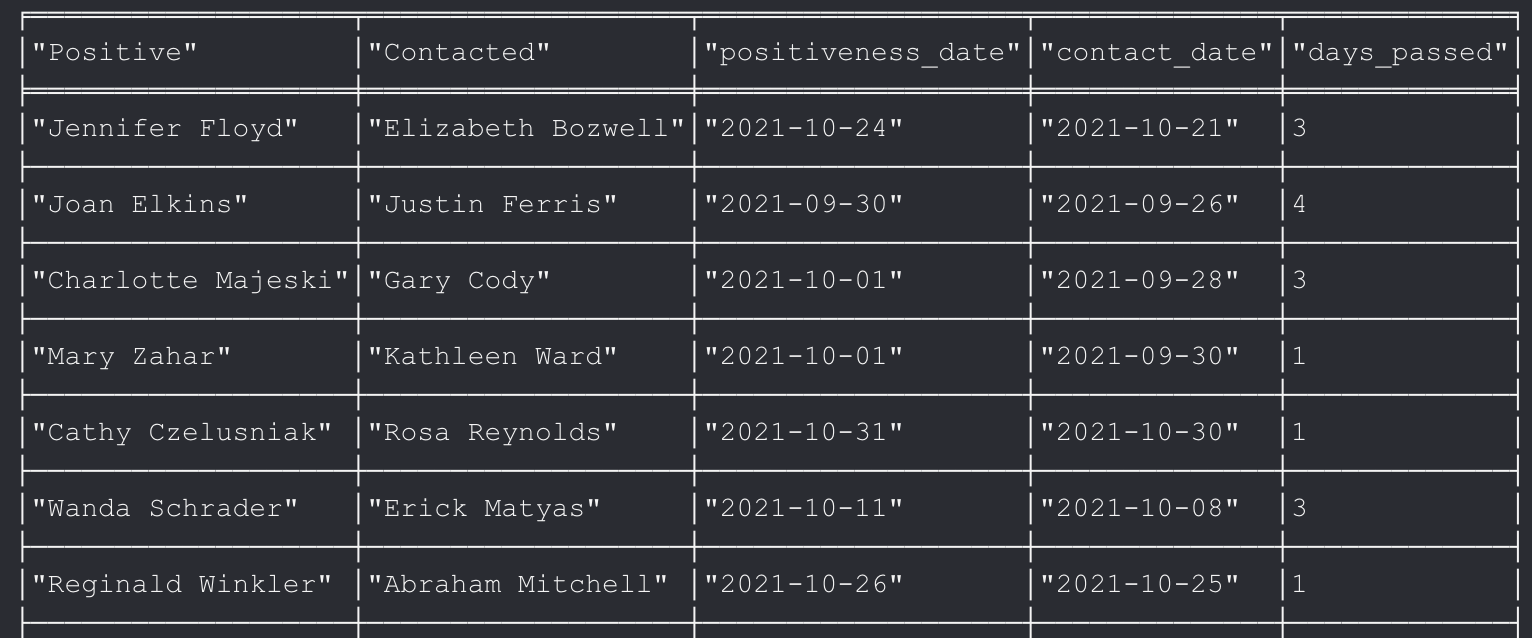
\includegraphics[width=\textwidth]{images/Query1.png}
\end{figure}
\subsubsection*{Query n. 2}
Find how many positive vaccinated people have a determined type of Vaccine, returning Positive to Total ratio
\begin{minted}
    [
    frame=lines,
    framesep=5mm,
    baselinestretch=1.5,
    escapeinside=||
    ]
    {mysql}
MATCH (m)-|[|:REGISTERED|]|->(c:Covid_Vaccines)
WITH c.|Type| as |Type|, count(*) as TotalNumber
ORDER BY c.|Type| 
MATCH (p:Person)-|[|:HAS|]|-(m:Medical_Record),
    (m)-|[|:REGISTERED|]|->(c:Covid_Vaccines)
WHERE p.Positive = True and |Type| = c.|Type|
RETURN  Type, count(*) as Positives, TotalNumber,
round(ToFloat(count(*)) / ToFloat(TotalNumber)*100, 2) + "%" as Percent 
ORDER BY Percent DESC
\end{minted}
\begin{figure}[H]
    \centering
    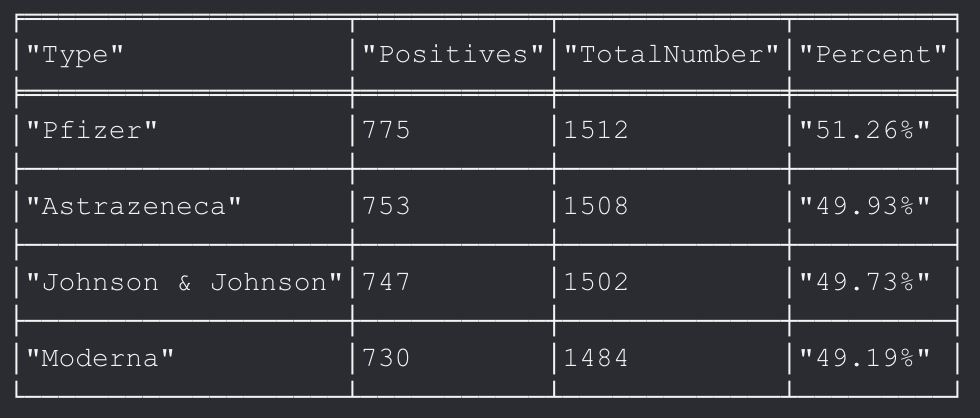
\includegraphics[width=\textwidth]{images/Query2.png}
\end{figure}
\subsubsection*{Query n. 3}
Find which places and rooms have been visited by positive person in the last 5 days for a duration time longer than 50 minutes
\begin{minted}
    [
    frame=lines,
    framesep=5mm,
    baselinestretch=1.5,
    escapeinside=||
    ]
    {mysql}
MATCH (p1:Person)-|[|v1:VISITS|]|->(pl:Place)
WHERE p1.Last_Confirm > v1.Date and 
    p1.Last_Confirm < v1.Date + duration(|{|days:5|}|)
    and
    p1.Positive = True and
    v1.Duration > time(|{|hour:0,minute:50|}|)
RETURN DISTINCT p1.CIF as CIF, p1.First_Name as Name, pl.Code as Place,
pl.Room as Room, v1.Date as Date,p1.Last_Confirm as Positiveness_Date
ORDER BY p1.CIF
UNION
MATCH (p1:Person)-|[|v1:VISITS|]|->(r:Rooms)
WHERE p1.Last_Confirm > v1.Date and 
    p1.Last_Confirm < v1.Date + duration(|{|days:5|}|)
    and
    p1.Positive = True and
    v1.Duration > time(|{|hour:0,minute:50|}|)
RETURN DISTINCT p1.CIF as CIF, p1.First_Name as Name, r.Code as Place, 
r.Name as Room, v1.Date as Date, p1.Last_Confirm as Positiveness_Date
ORDER BY p1.CIF
\end{minted}
\begin{figure}[H]
    \centering
    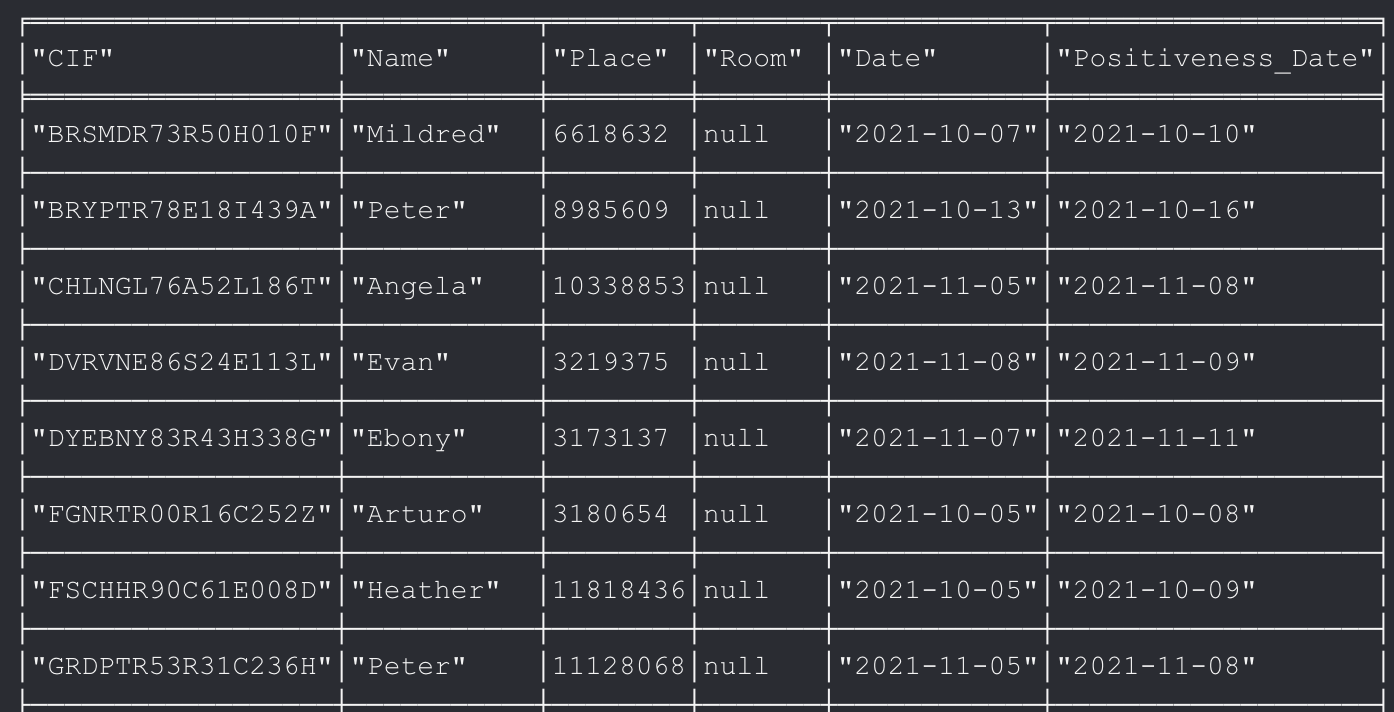
\includegraphics[width=\textwidth]{images/Query3.png}
\end{figure}
\newpage
\subsubsection*{Query n. 4}
Track all the people who were in contact with a positive in the last 15 days from his confirmation and find all their familiars
\begin{minted}
    [
    frame=lines,
    framesep=5mm,
    baselinestretch=1.5,
    escapeinside=||
    ]
    {mysql}
MATCH (p1:Person|{|Positive:true|}|)-|[|c:CONTACTS|]|-(p2:Person)
WHERE p1.Last_Confirm >= c.Date and p1.Last_Confirm <= c.Date + duration(|{|days: 15|}|)
MATCH (p2)-|[|:LIVES*|]|-(p4:Person), (p1)-|[|:LIVES*|]|-(p3:Person)
RETURN DISTINCT p1, p2, p3, p4
\end{minted}
\begin{figure}[H]
    \centering
    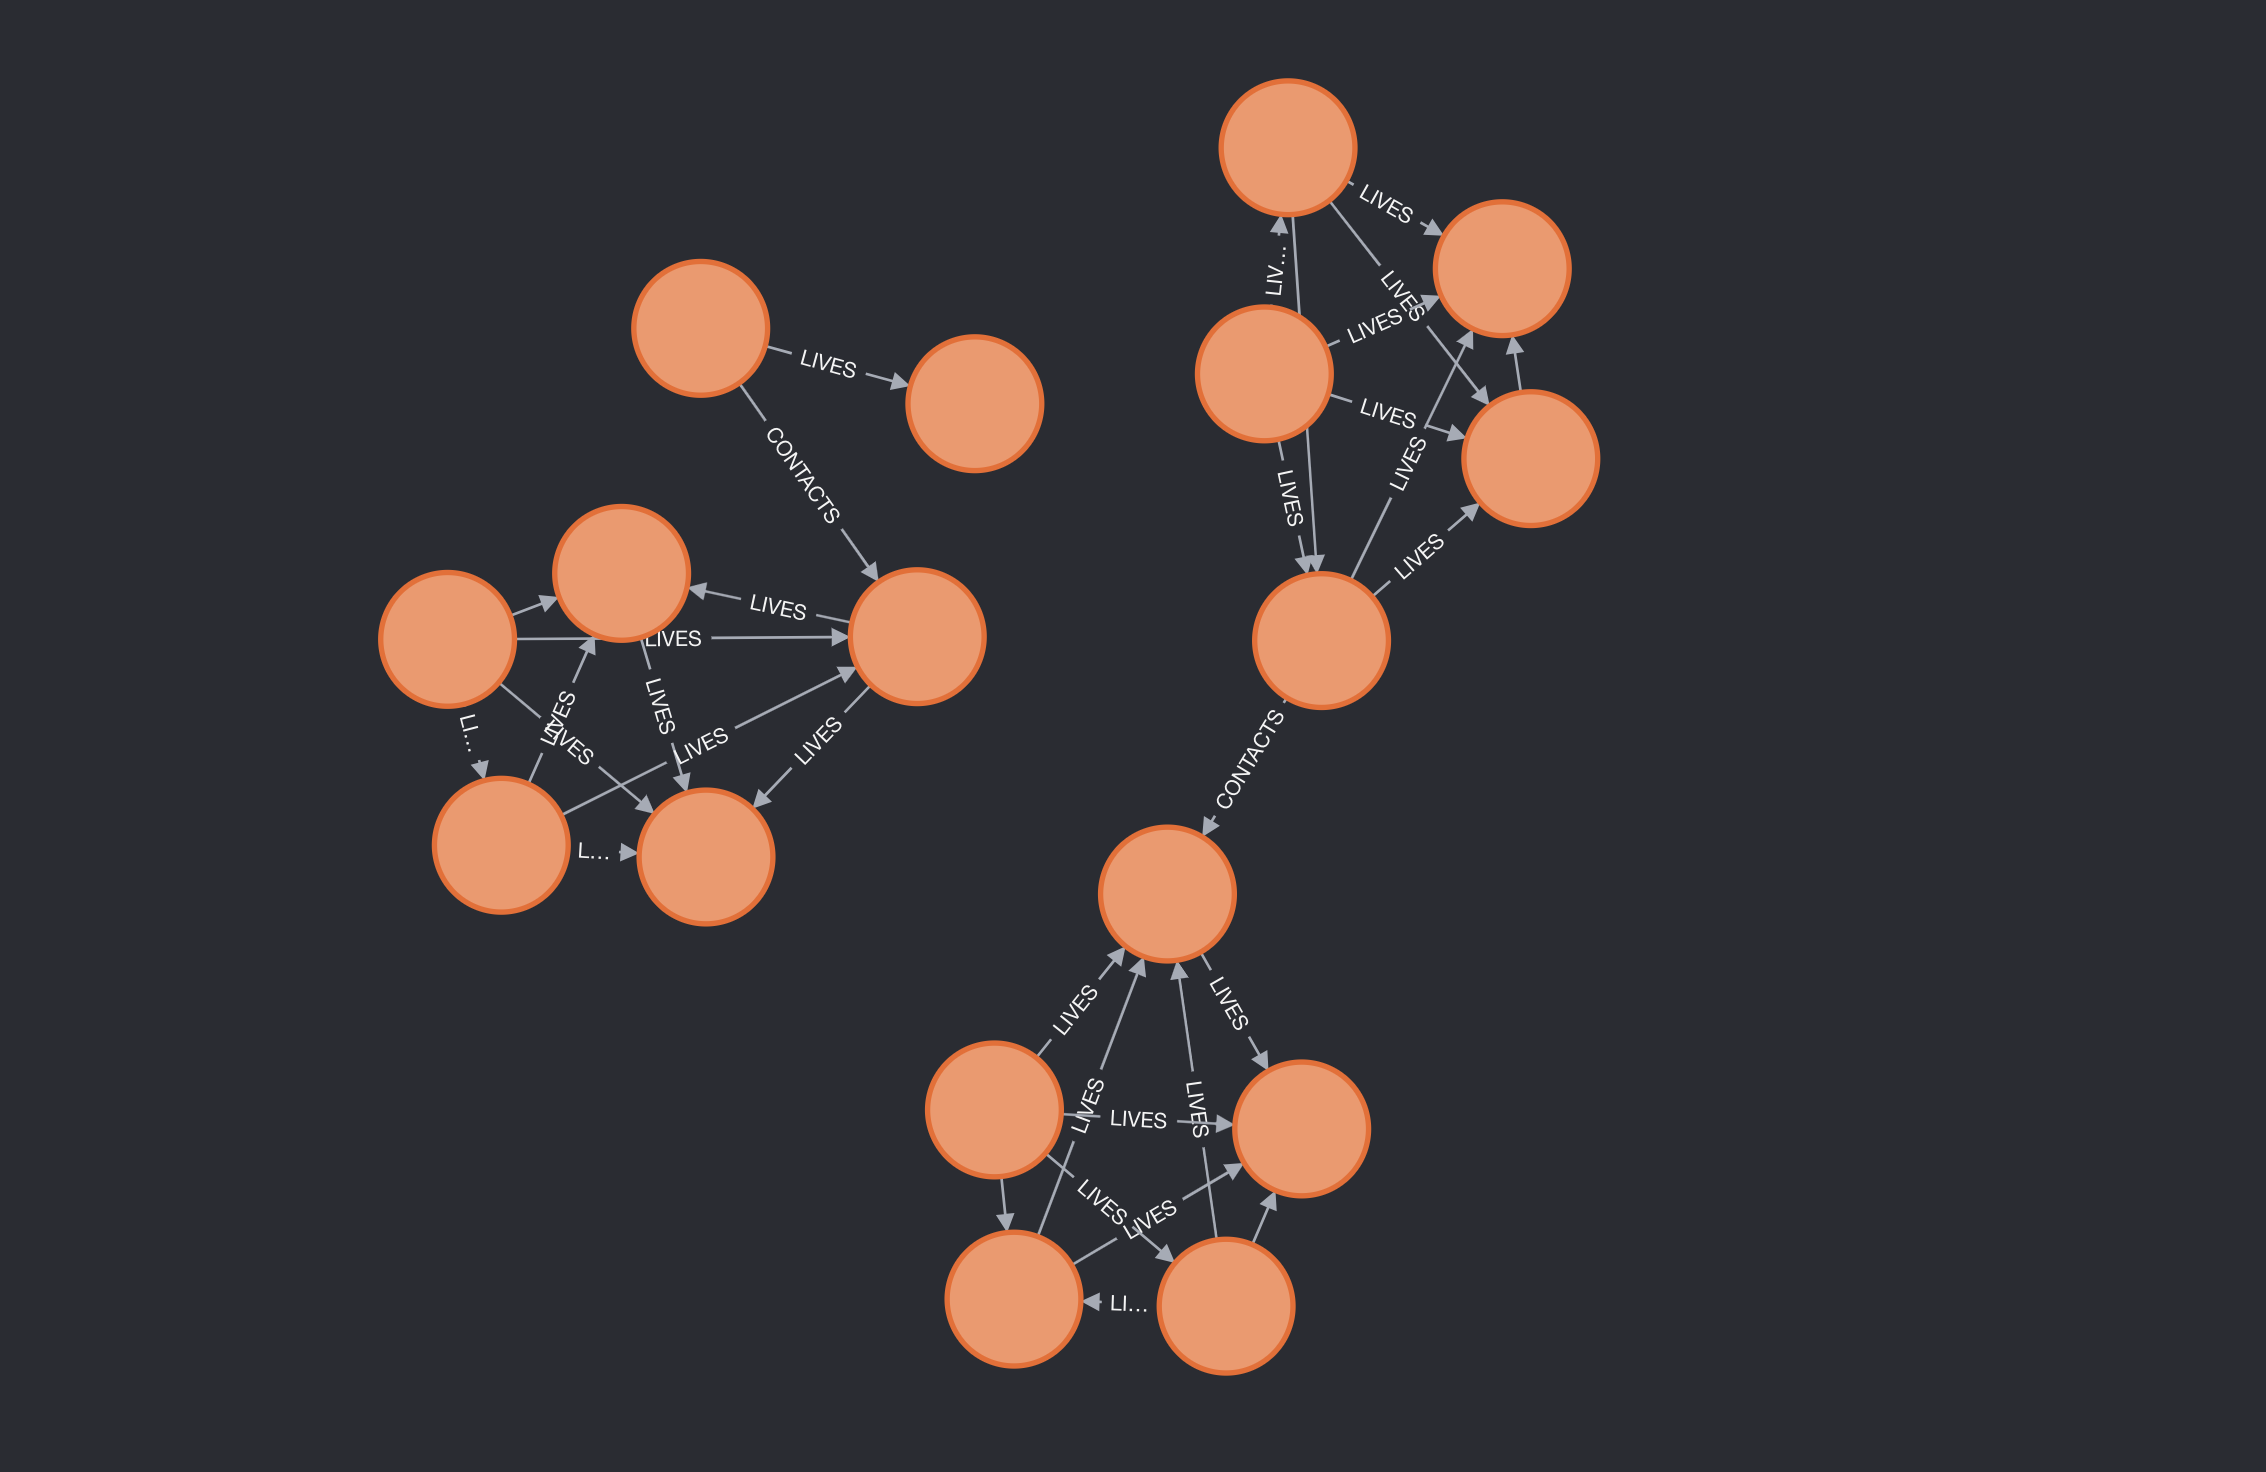
\includegraphics[width=\textwidth]{images/Query4.png}
\end{figure}
\subsubsection*{Query n. 5}
Track all the people who were in the same place of a positive in the last 15 days from his confirmation
\begin{minted}
 [
    frame=lines,
    framesep=5mm,
    baselinestretch=1.5,
    escapeinside=||
    ]
    {mysql}
MATCH (p1:Person|{|Positive:true|}|)-|[|v1:VISITS|]|->(pl:Place)<-|[|v2:VISITS|]|-(p2:Person) 
WHERE p1.Last_Confirm >= v1.Date and p1.Last_Confirm >= v2.Date and 
p1.Last_Confirm <= v1.Date + duration(|{|days: 15|}|) and 
p1.Last_Confirm <= v2.Date + duration(|{|days: 15|}|)
RETURN DISTINCT p1.First_Name + " " + p1.Last_Name as Positive, 
p2.First_Name + " " + p2.Last_Name as Contacted, pl.Name as Place, p1.Last_Confirm, 
v1.Date as Positive_Visit, v2.Date as Contact_Visit
\end{minted}
\begin{figure}[H]
    \centering
    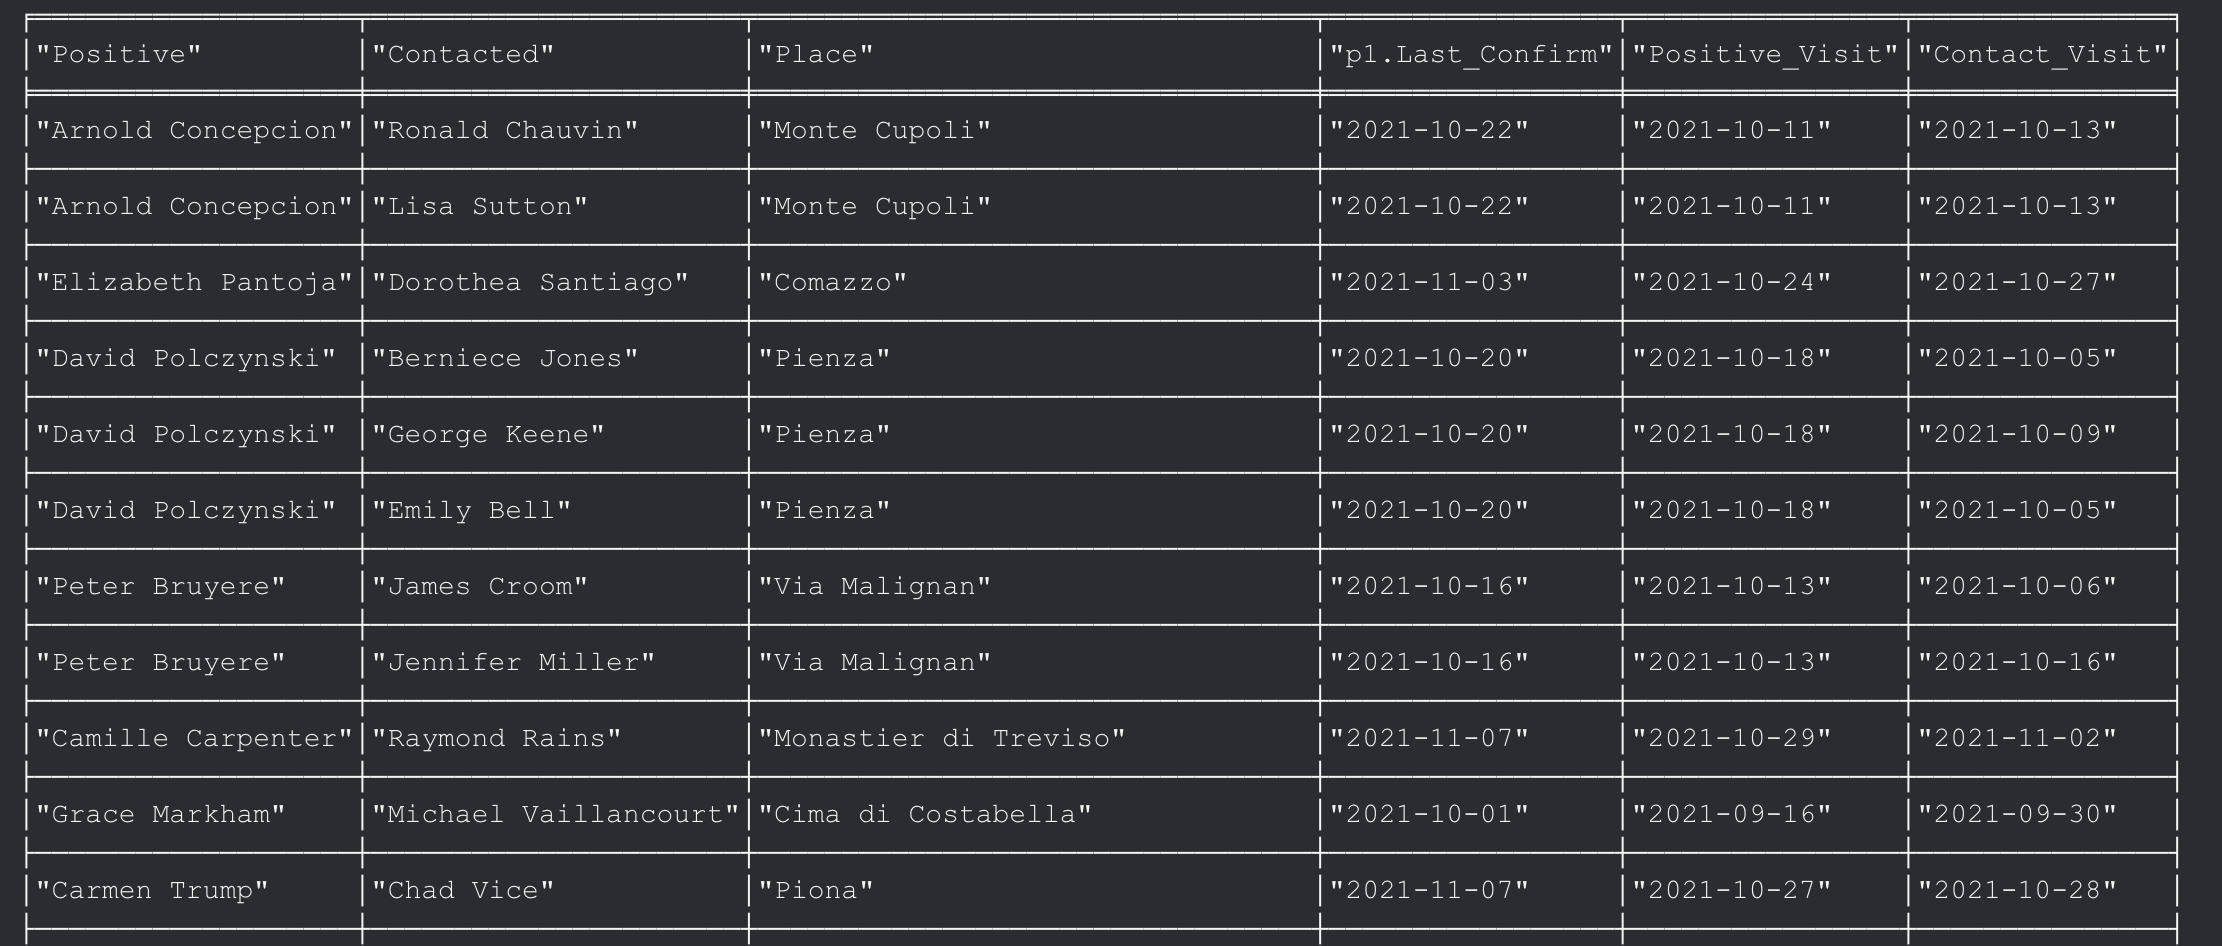
\includegraphics[width=\textwidth]{images/Query5.png}
\end{figure}
\subsubsection*{Query n. 6}
Track all the people who were in contact, also indirectly, with a positive or with one of his contacts in the last 15 days of his confirmation. \\The possible infected are risky subjects and they don't have a vaccine
\begin{minted}
 [
    frame=lines,
    framesep=5mm,
    baselinestretch=1.5,
    escapeinside=||
    ]
    {mysql}
MATCH p = (p1:Person|{|Positive:true|}|)-|[|*|]|-(p2:Person)
WHERE ALL(r IN relationships(p) WHERE (p1.Last_Confirm >= r.Date and 
p1.Last_Confirm <= r.Date + duration(|{|days: 15|}|)))
MATCH (p2:Person)-|[|:HAS|]|->(m:Medical_Record|{|Risky_Subject:true|}|)
WHERE NOT (m)-|[|:REGISTERED|]|->(:Covid_Vaccines)
RETURN DISTINCT p1.First_Name + " " + p1.Last_Name as Positive, 
p2.First_Name + " " + p2.Last_Name as Contacted, p1.Last_Confirm, p
\end{minted}
\begin{figure}[H]
    \centering
    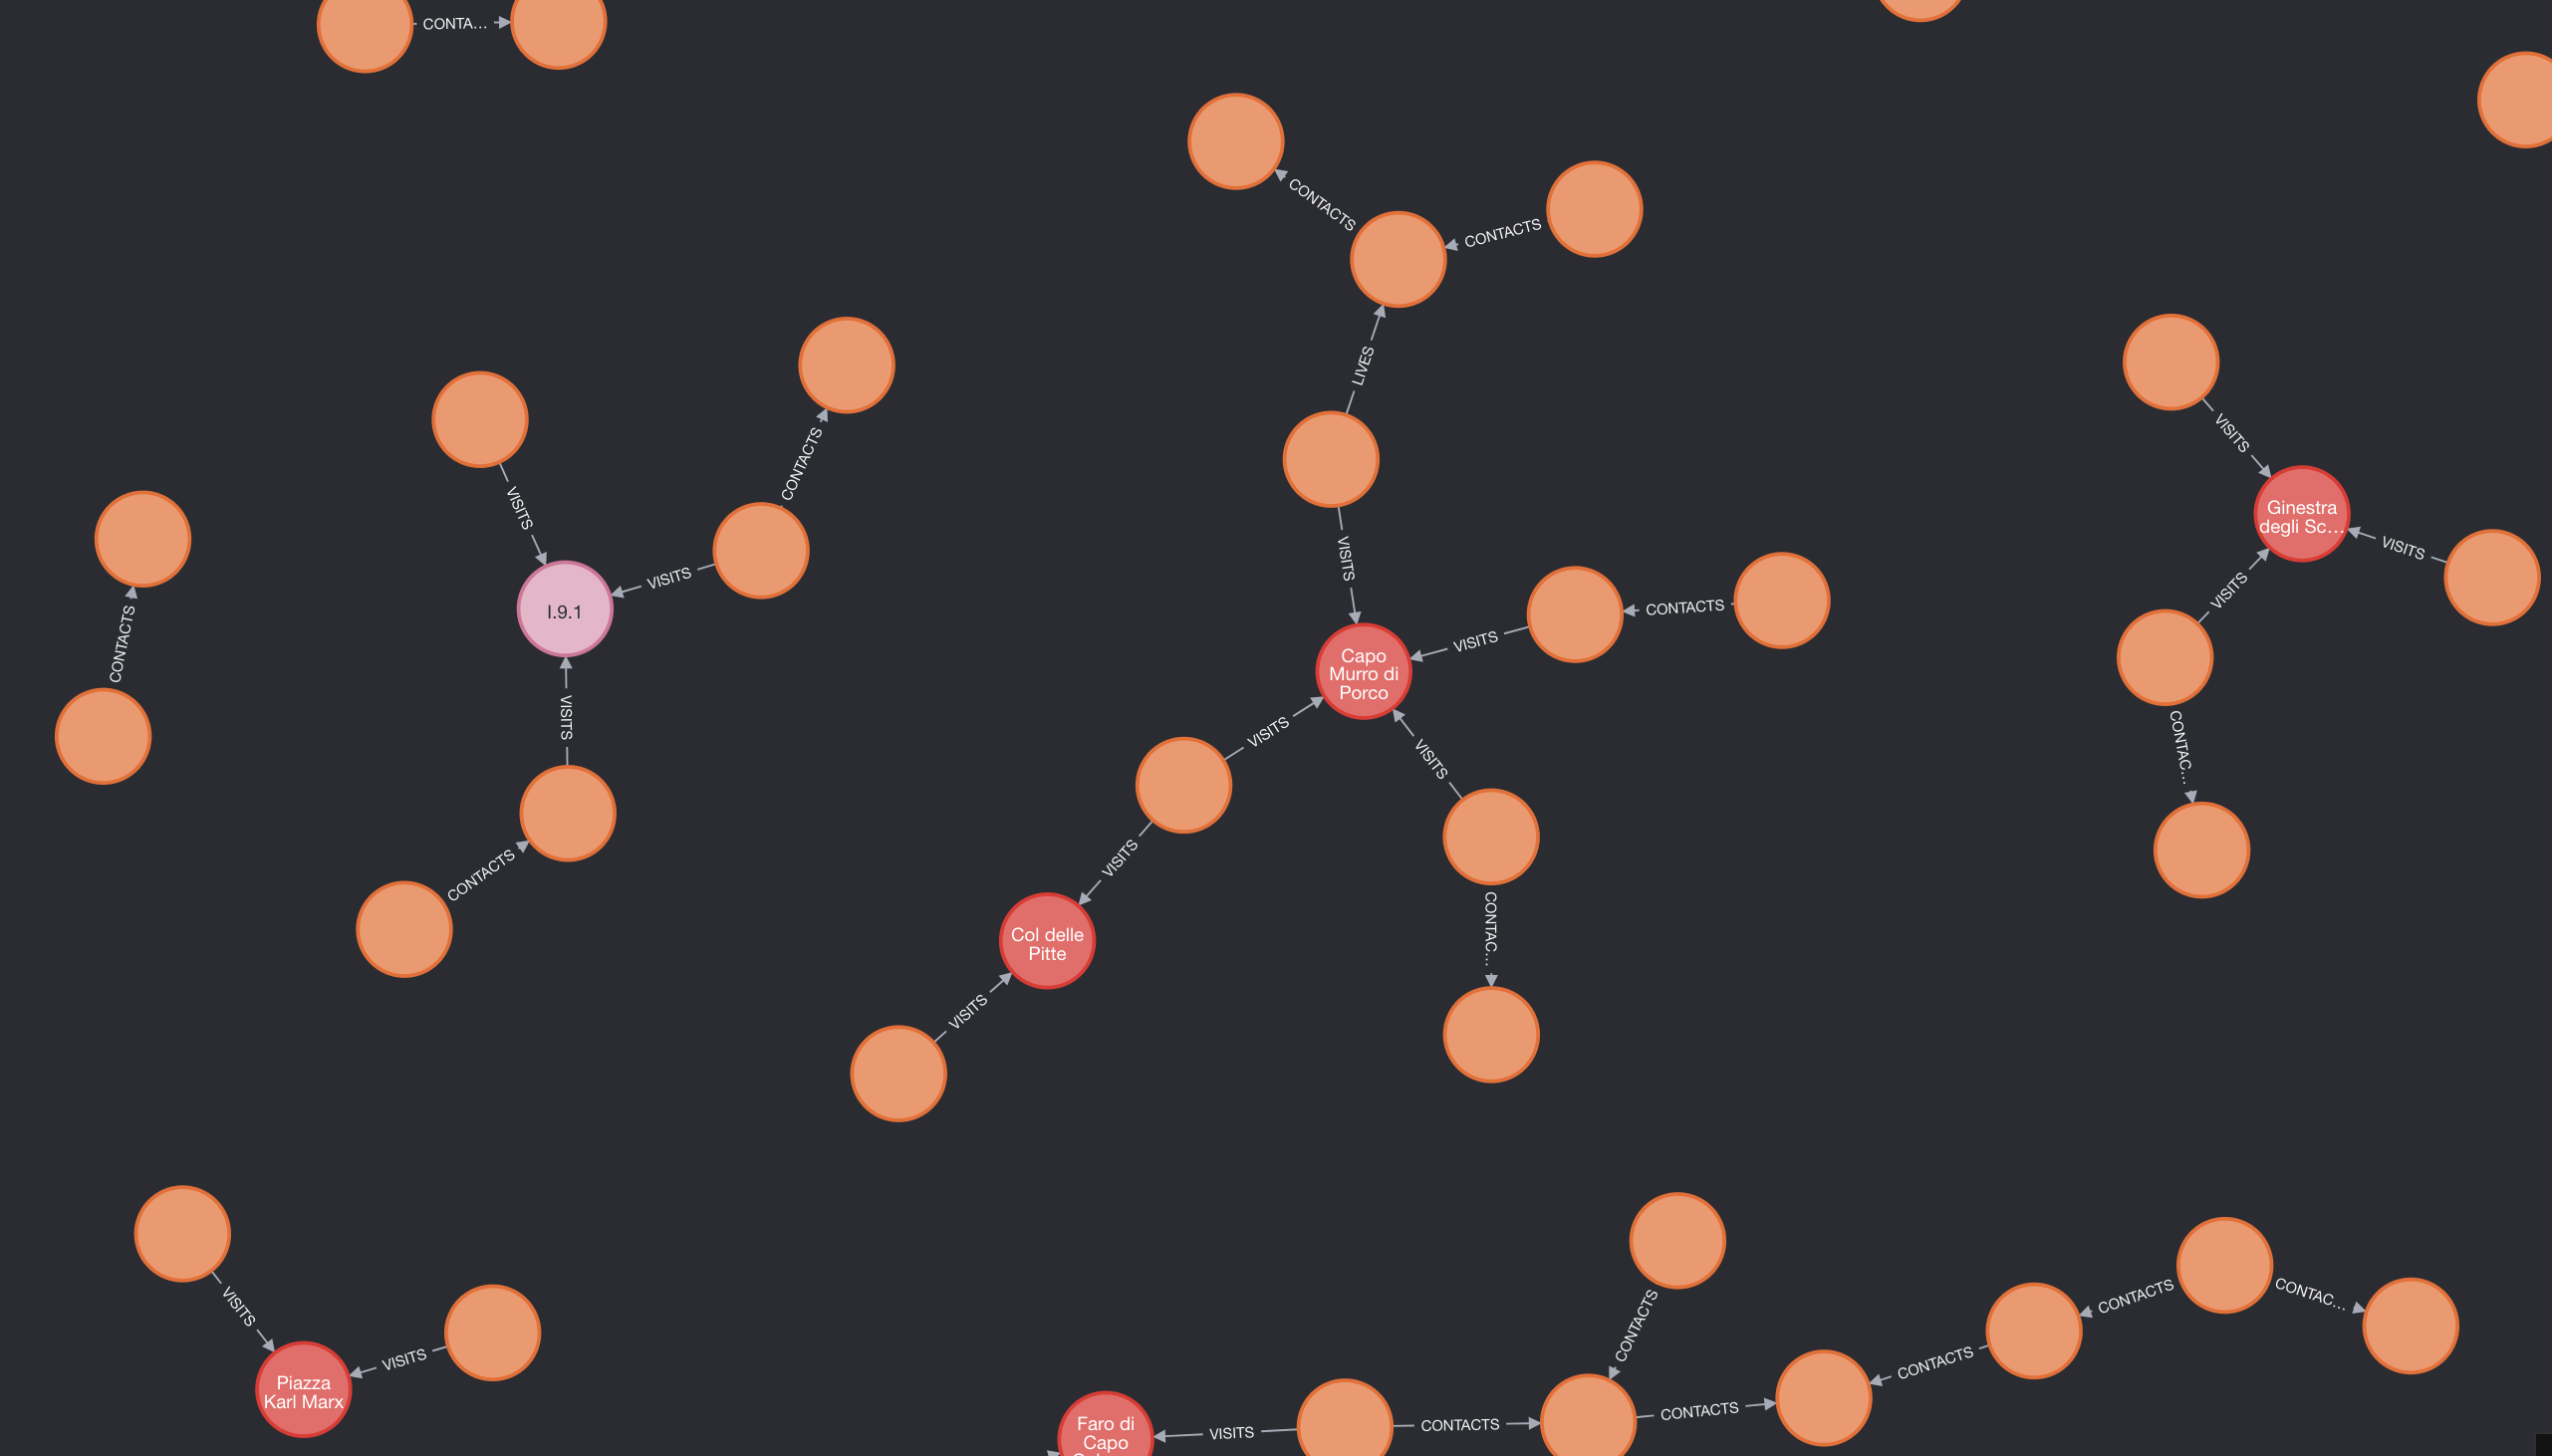
\includegraphics[width=\textwidth]{images/Query6.png}
\end{figure}
\subsubsection*{Query n. 7}
Given two people, one positive and one negative, find the shortest path for which they could have been in contact
The negative person has only vaccine and he hasn't done a test in the last 2 days from the positive confirmation.
\begin{minted}
 [
    frame=lines,
    framesep=5mm,
    baselinestretch=1.5,
    escapeinside=||
    ]
    {mysql}
MATCH (p1:Person|{|Positive: true|}|), (p2:Person|{|Positive:false|}|), 
p = shortestPath((p1)-|[|*|]|-(p2))
WHERE ALL(r IN relationships(p) WHERE (p1.Last_Confirm >= r.Date and 
p1.Last_Confirm <= r.Date + duration(|{|days: 15|}|))) 
MATCH (p2)-|[|:HAS|]|->(m:Medical_Record), (m)-|[|:REGISTERED|]|->(t:Covid_Tests), 
(m)-|[|r:REGISTERED|]|->(v:Covid_Vaccines)
WITH p1, p2, max(t.Date) as Max_Date, count(v) as nv
WHERE (p1.Last_Confirm >= Max_Date and
p1.Last_Confirm > Max_Date + duration(|{|days: 2|}|)) and 
nv=1
RETURN DISTINCT p1.First_Name + " " + p1.Last_Name as Positive, 
p2.First_Name + " " + p2.Last_Name as Negative, p1.Last_Confirm, 
Max_Date as Latest_Test
\end{minted}
\begin{figure}[H]
    \centering
    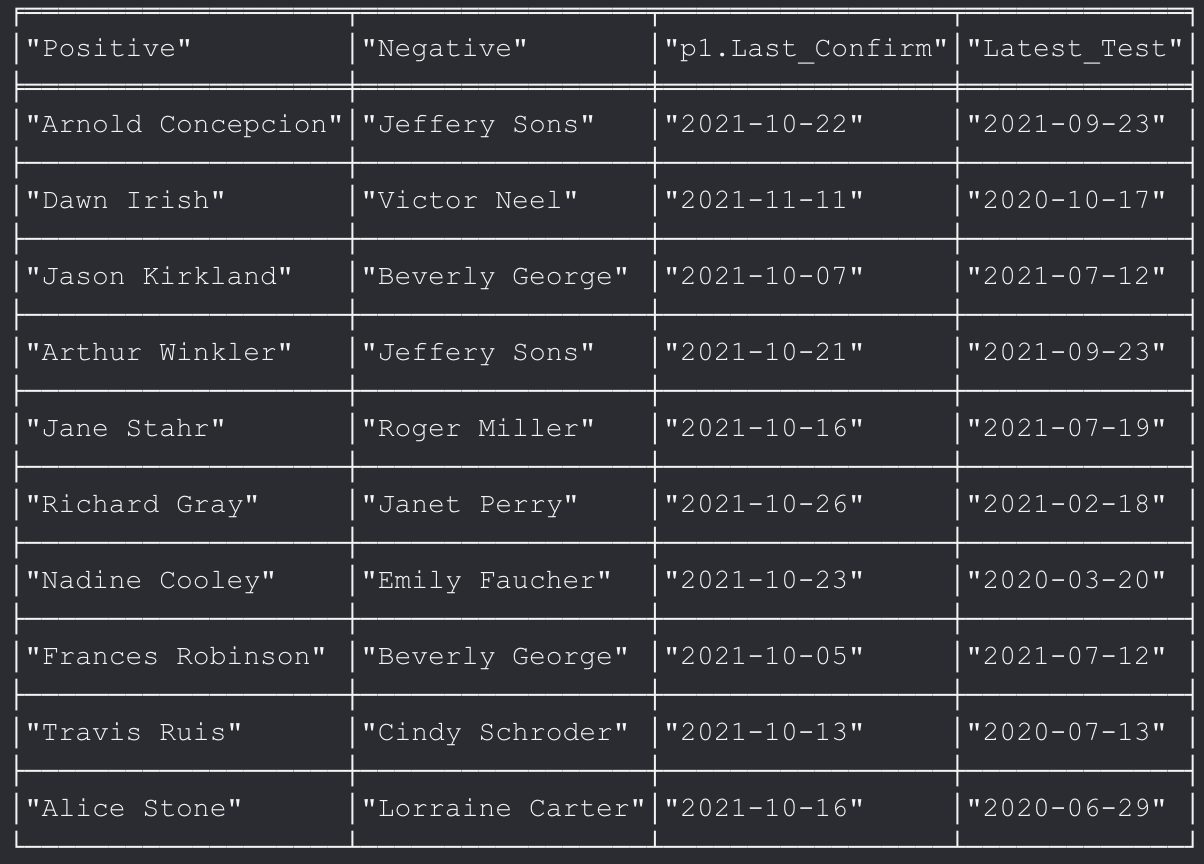
\includegraphics[width=\textwidth]{images/Query7.png}
\end{figure}
%%%%%%%%%%%%%%%%%%%%%%%%%%%%%%%%%%%%%%%%%%%%%%%%%%%%%%%%%%%%%%%%%
\subsubsection{Query n. 8}
Find all the connection a positive person had, returning nodes for graphical representation.
\begin{minted}
 [
    frame=lines,
    framesep=5mm,
    baselinestretch=1.5,
    escapeinside=||
    ]
    {mysql}
MATCH(p:Person)
WITH p, p.Last_Confirm as P_Date, duration(|{|days:50|}|) as TimeElapsed
MATCH relation_1 = (p)-|[|v1:VISITS|]|->(pl:Place)<-|[|v3:VISITS|]|-(:Person)
WHERE (P_Date > v1.Date and P_Date < v1.Date + TimeElapsed) and 
(P_Date > v3.Date and P_Date < v3.Date + TimeElapsed) and
(v1.Date >  v3.Date and v1.Date  < v3.Date + TimeElapsed)
WITH p, P_Date, relation_1, TimeElapsed
MATCH relation_2 = (p)-|[|v2:VISITS|]|->(r:Rooms)<-|[|v4:VISITS|]|-(:Person)
WHERE(P_Date > v2.Date and P_Date < v2.Date + TimeElapsed) and 
(P_Date > v4.Date and P_Date < v4.Date + TimeElapsed) and
(v2.Date >  v4.Date and v2.Date  < v4.Date + TimeElapsed)
WITH p, P_Date, relation_1, relation_2, TimeElapsed
MATCH relation_3 = (p)-|[|c:CONTACTS|]|->(:Person)
WHERE (P_Date > c.Date and P_Date < c.Date + TimeElapsed)
WITH p, P_Date, relation_1, relation_2, relation_3, TimeElapsed
MATCH relation_4 = (p)-|[|:LIVES|]|->(:Person)
RETURN relation_1, relation_2, relation_3, relation_4
\end{minted}
\begin{figure}[H]
    \centering
    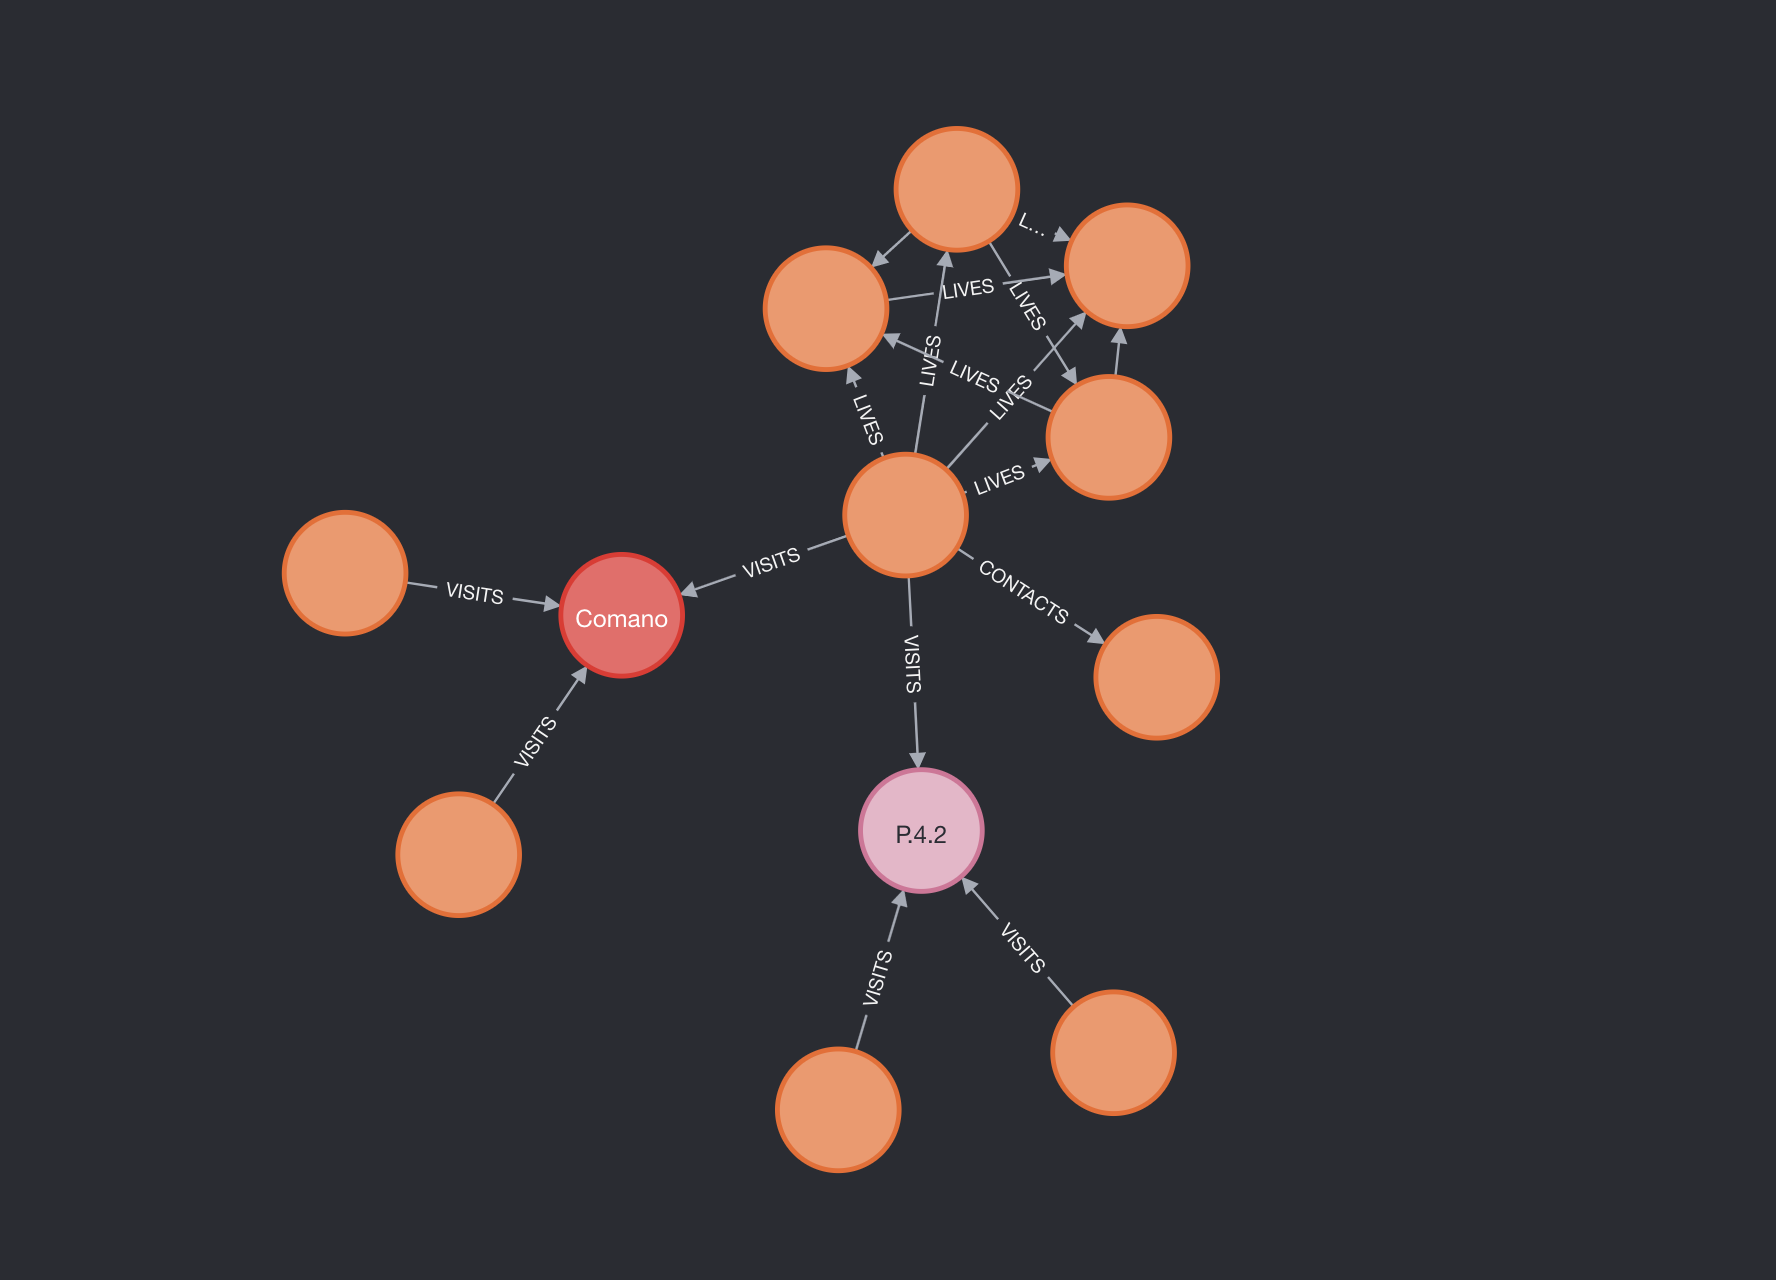
\includegraphics[width=\textwidth]{images/Query8.png}
\end{figure}
\newpage
\subsection{Commands}
Below some commands that manipulates the database. \\ 
(NOTE) The nodes generated with "generate\_dataset.py" are coerent with the assumptions, in order to get some corrupted CSV files, use "generate\_inconsistent\_dataset.py"
\subsubsection{Command n. 1}
If a person has done at least 1 vaccine, set his Vaccinated attribute to true
\begin{minted}
 [
    frame=lines,
    framesep=5mm,
    baselinestretch=1.5,
    escapeinside=||
    ]
    {mysql}
MATCH (p:Person)-|[|:HAS|]|->(m:Medical_Record), (m)-|[|:REGISTERED|]|->(v:Covid_Vaccines) 
SET m.Covid_Vaccinated=True
RETURN DISTINCT m, v
\end{minted}
\begin{figure}[H]
    \centering
    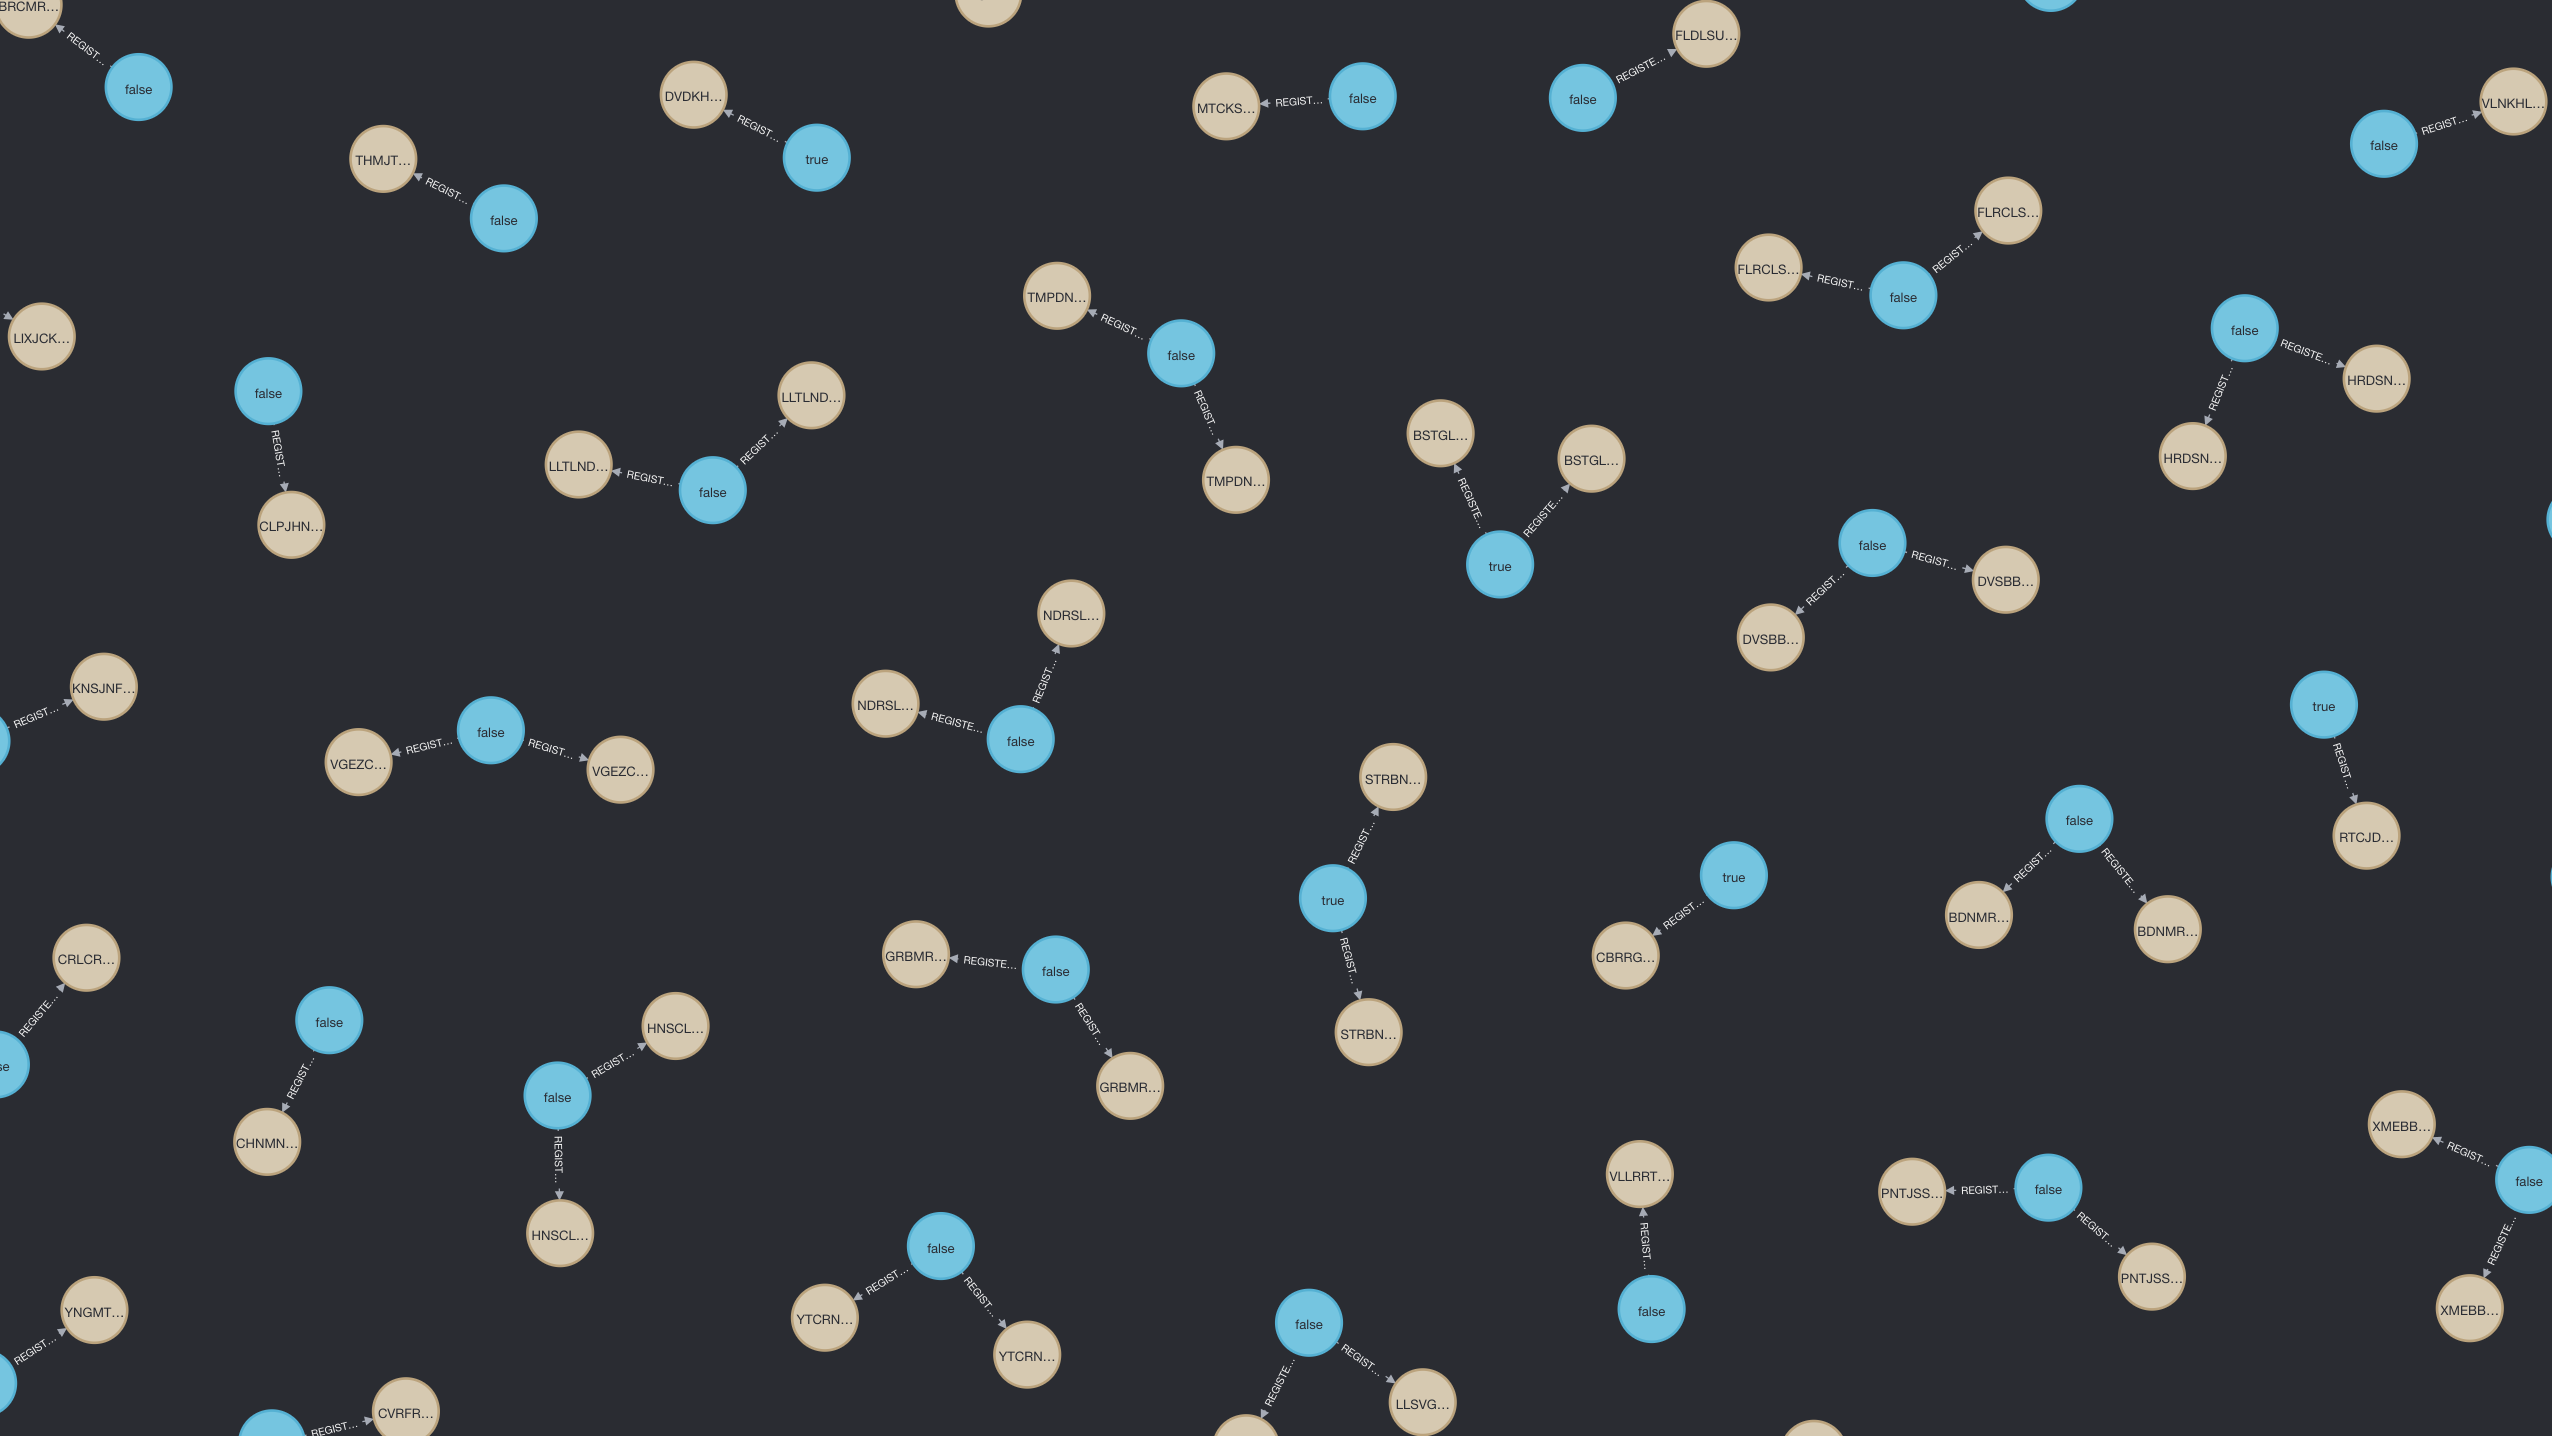
\includegraphics[width=\textwidth]{images/Command1.png}
\end{figure}
\subsubsection{Command n. 2}
If a person results negative in his latest test then set is Positive attribute to false.
\begin{minted}
 [
    frame=lines,
    framesep=5mm,
    baselinestretch=1.5,
    escapeinside=||
    ]
    {mysql}
MATCH (p:Person)-|[|:HAS|]|->(m:Medical_Record), (m)-|[|:REGISTERED|]|->(t:Covid_Tests)
WITH p, max(t.Date) as Max_Date
MATCH(p)-|[|:HAS|]|->(m:Medical_Record), (m)-|[|:REGISTERED|]|->(t:Covid_Tests)
WHERE t.Date = Max_Date and t.Result=False
SET p.Positive = False
RETURN p, m, t
\end{minted}
\begin{figure}[H]
    \centering
    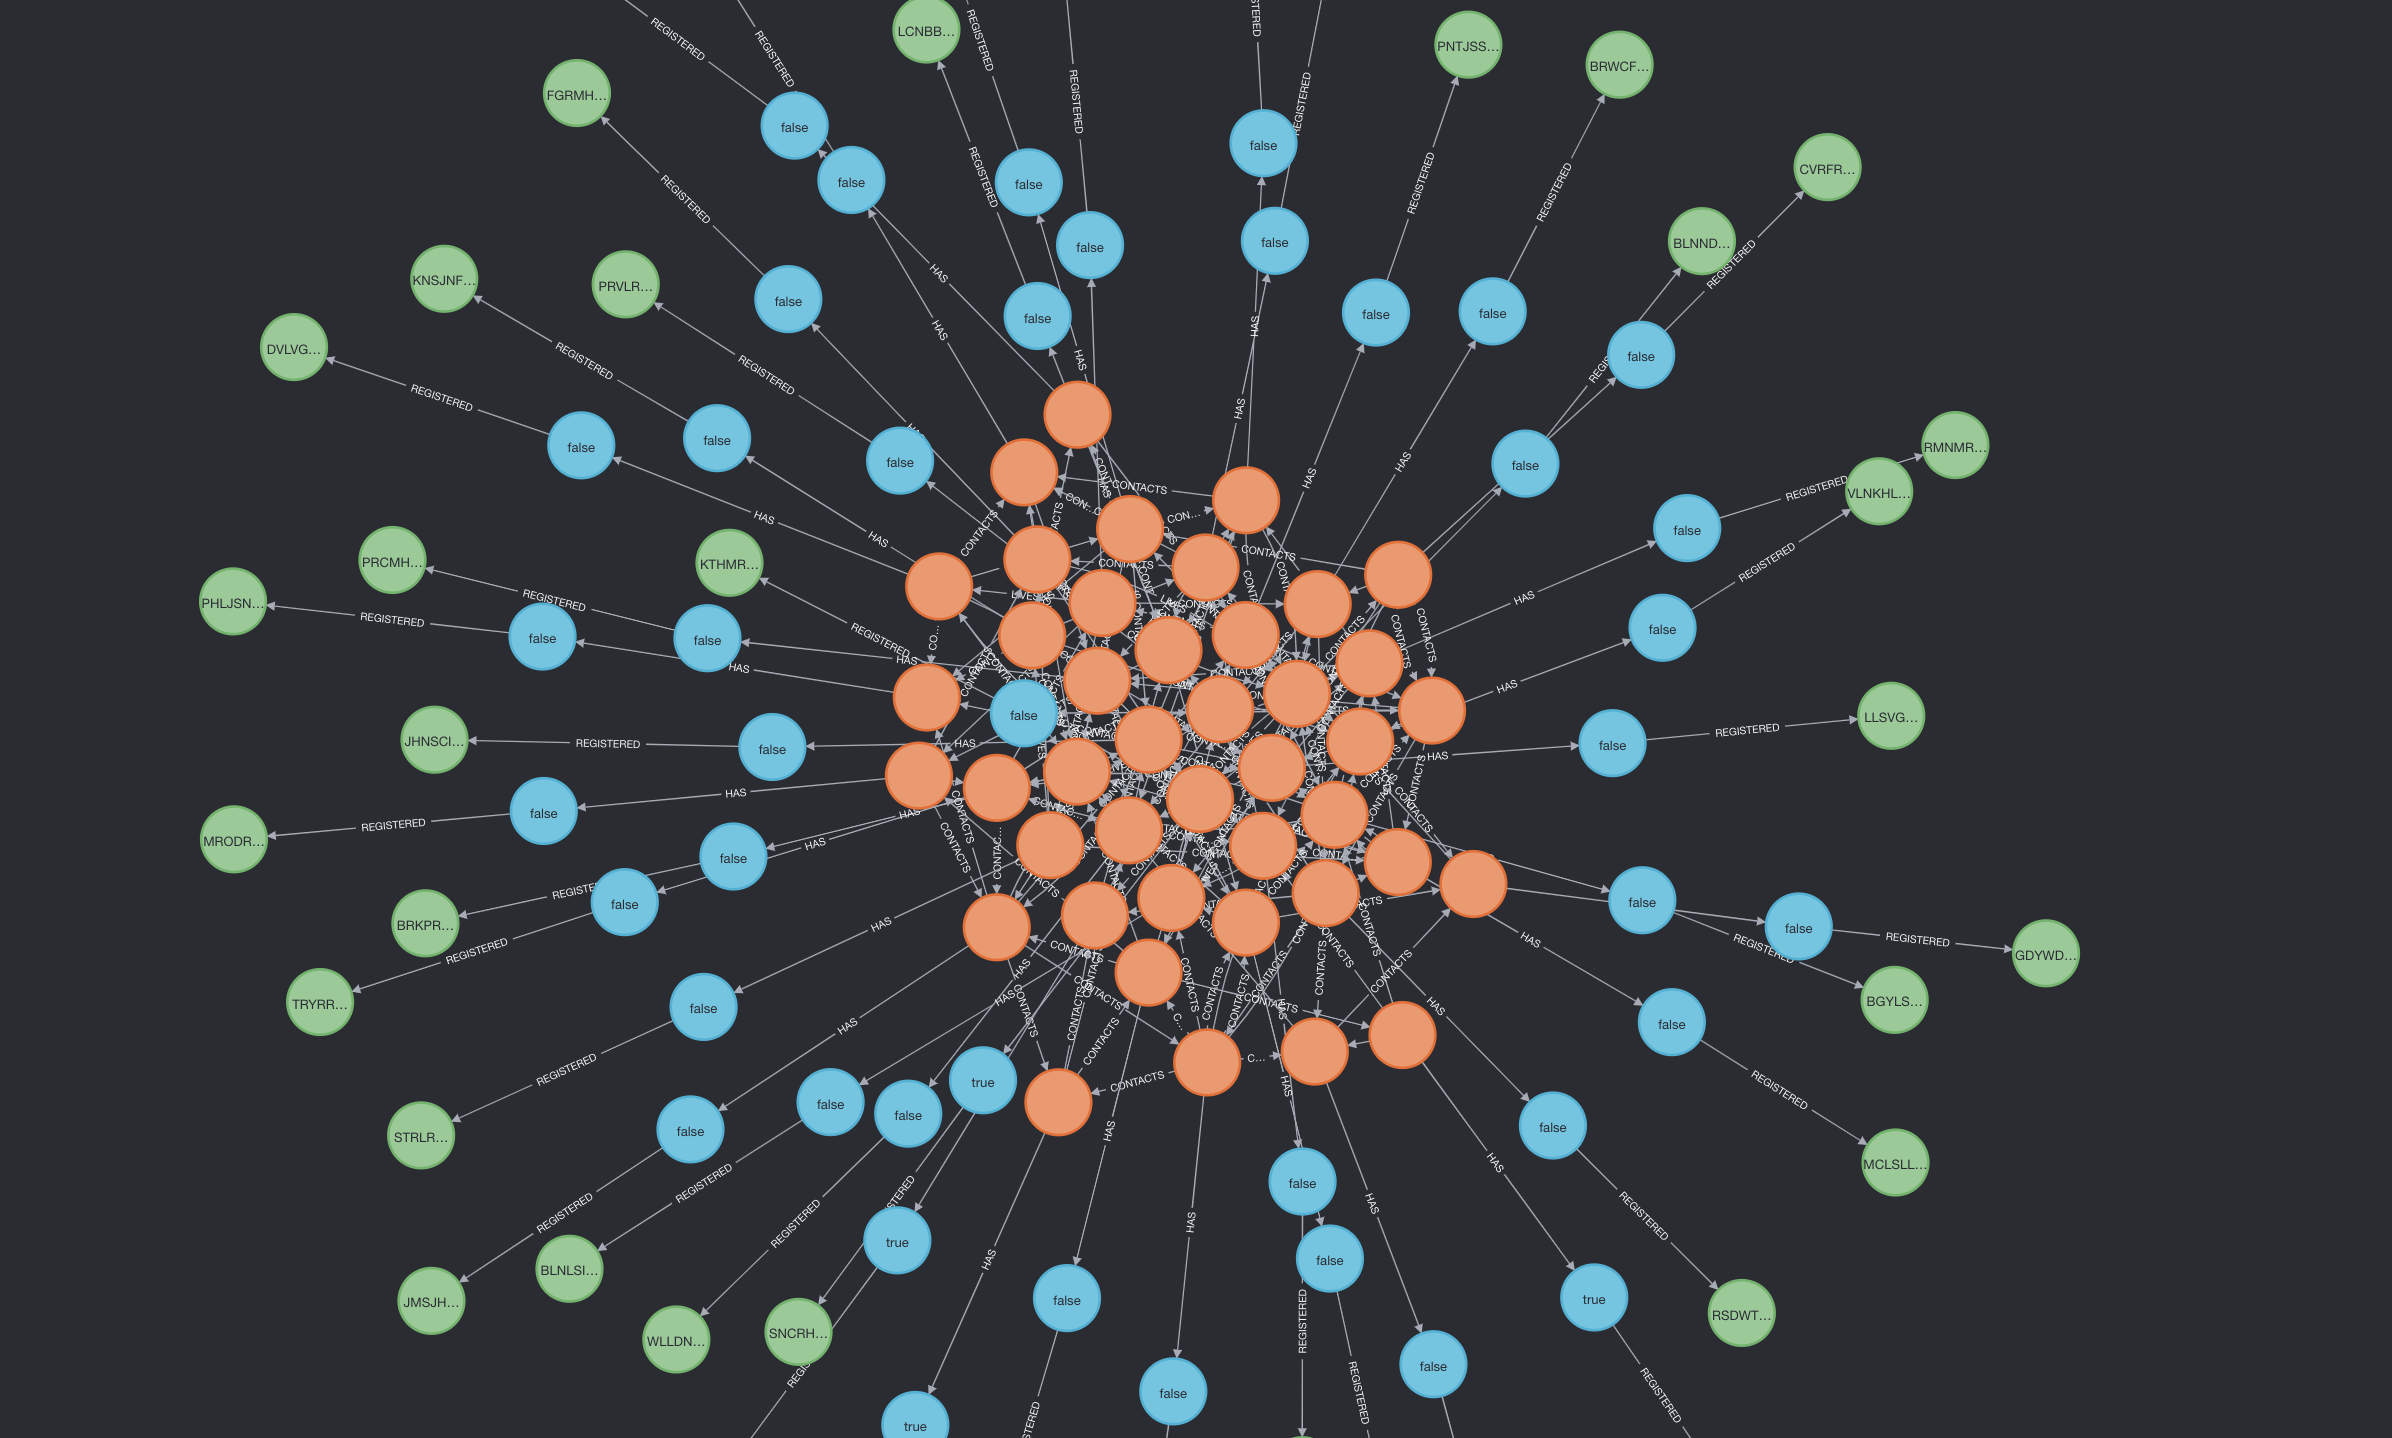
\includegraphics[width=\textwidth]{images/Command2.png}
\end{figure}


\subsubsection{Command n. 3}
Delete all rooms never visited from any person  
\begin{minted}
 [
    frame=lines,
    framesep=5mm,
    baselinestretch=1.5,
    escapeinside=||
    ]
    {mysql}
MATCH (r:Rooms)
WHERE NOT (:Person)-|[|:VISITS|]|-(r)
DETACH DELETE r
\end{minted}
\begin{figure}[H]
    \centering
    
\includegraphics[width=\textwidth]{images/Command3.png}
\end{figure}
\subsubsection{Command n. 4}
Delete all people without medical record  
\begin{minted}
 [
    frame=lines,
    framesep=5mm,
    baselinestretch=1.5,
    escapeinside=||
    ]
    {mysql}
MATCH (p:Person)
WHERE NOT (p)-|[|:HAS|]|->(:Medical_Record)
DETACH DELETE p
\end{minted}
\begin{figure}[H]
    \centering
    
\includegraphics[width=\textwidth]{images/Command4.png}
\end{figure}


\section{User Interface Implementation}
The user interface was centered around 3 pillars:
\begin{enumerate}
    \item \textbf{Simplicity.} We set out to build a simple, streamlined web application, in order to gain familiarity with the tools that interact with Neo4J. That said, we wanted to avoid increasing the complexity of the project, so we strove to keep it as straight forward as possible.
    \item \textbf{Usefulness.} Although the User Interface is simple, it is not useless. In this context, we decided our measure of utility would not be a "commercial" one, like the value one could generate from our product, but the knowledge we would gain by building it.
    \item \textbf{UX.} Because of the simplicity of the webapp, we thought the least we could do was to make it easy to use. We hope we succeeded!
\end{enumerate}
The UI is divided into 3 sections: in the top left, the query list is available. Each one has a description hidden under a collapsable pane, a simple button to run it and a name. In the bottom left, we included a way to run personalized queries, leaving it to the user if they wanted to see the result as a graph, or as a table. Lastly, on the right half of the screen, either a graph or a table collecting results is shown.
\begin{figure}[H]
    \centering
    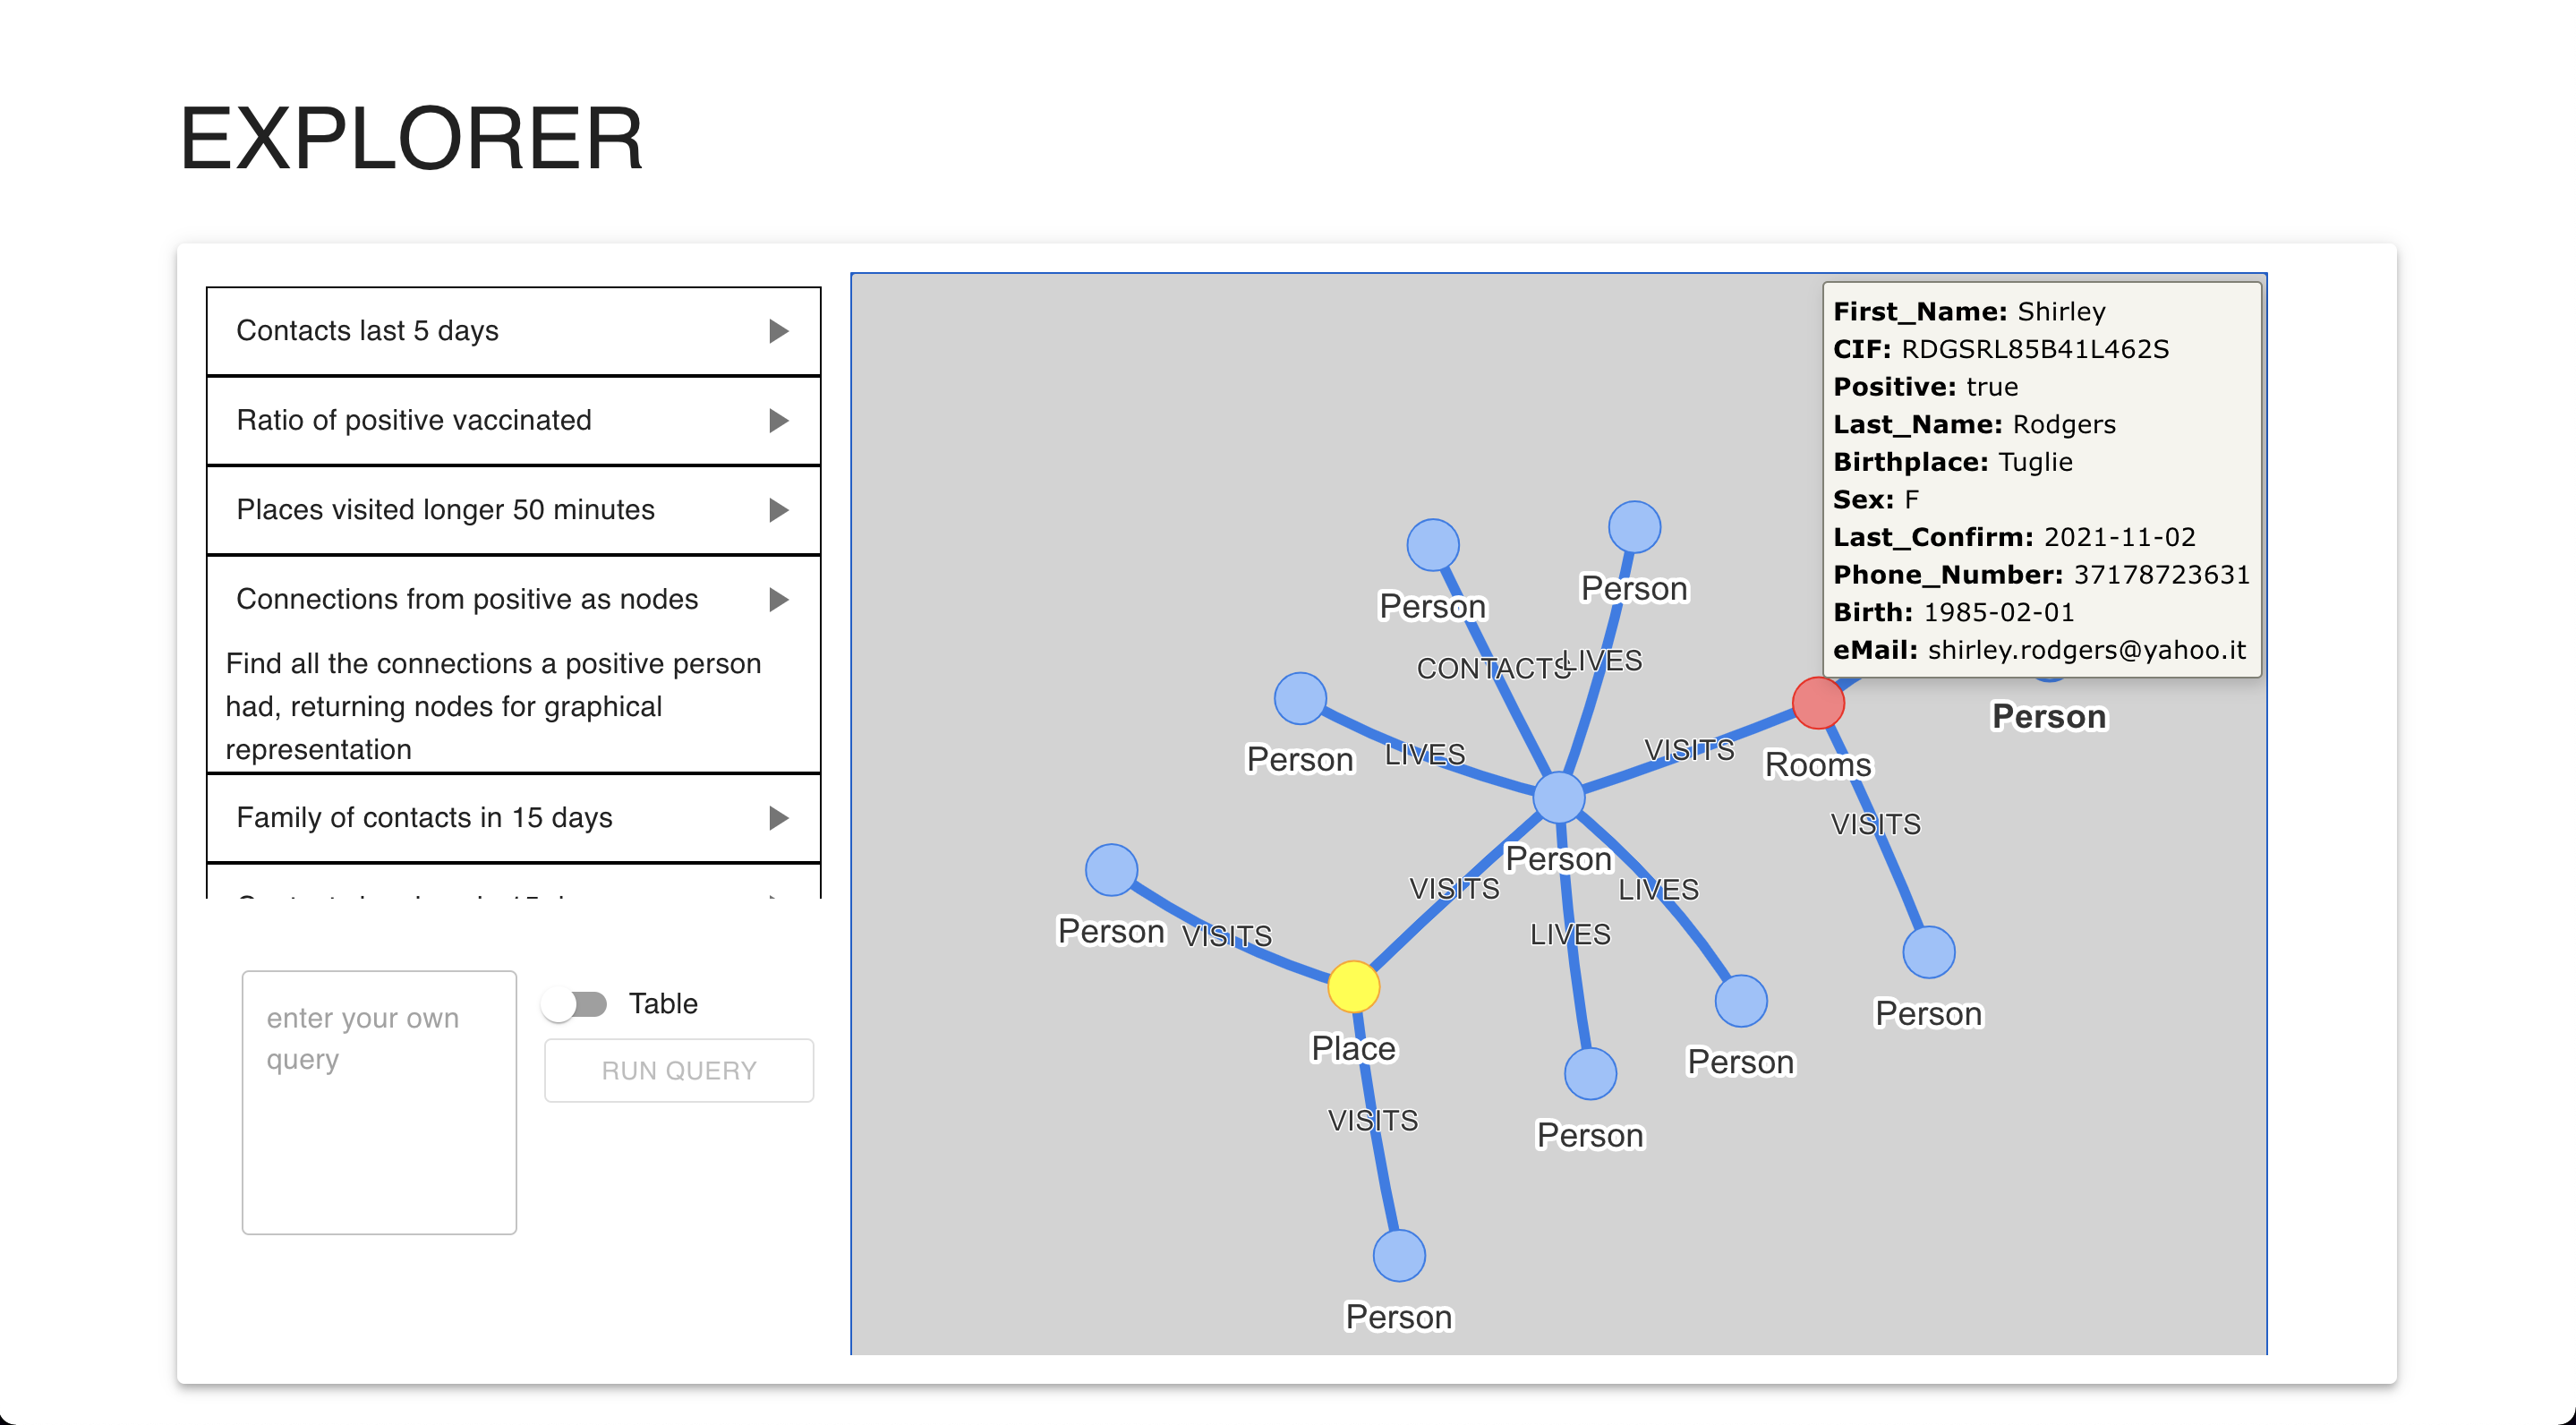
\includegraphics[width=\textwidth]{images/UI1.png}
\end{figure}

The tools we leveraged to code it are:
\begin{enumerate}
    \item \textbf{React.} We believe it needs no introduction; one of our project members had already worked with it, so we decided to leverage his experience to fast-forward development.
    \item \textbf{Material UI.} We needed a simple, preconfigured library for common UI elements, with React components included out of the box.
    \item \textbf{Use-Neo4J.} Luckily, we weren't the first one to bind a React application to a Neo4J database (considering the popularity of the GRANDstack, this wasn't news to us). We used this simple library to manage drivers and simplify our code.
    \item \textbf{NeoVis.js} This simple repo wraps a Neo4J driver together with a vis.js visualization method; because of version clashing, we were forced to use an older version, which didn't allow us to use an external driver; this means some of our requests are doubled.
\end{enumerate}



%%%%%%%%%%%%%%%%%%%%%%%%%%%%%%%%%%%%%%%%%%%%%%%%%%%%%%%%%%%%%%%%%

\section{Conclusion and possible improvements}
In this report, we outlined design and implementative choices behind the first part of the SAMBUD Fall 2021 project at Polimi.
The project has been very interesting both from the theoretical part and the practical part. From the practical point of view it has permitted to understand better and elaborate on Neo4j and Cypher. From the theoretical point of view it has been an interesting challenge to create an ER model and then a graph database that could be used to reason on a real problem. It was interesting working on the differences between a relational database and a graph database mostly thanks to the features of a graph. The queries were created to be easy to understand but also trying to use and highlight the potential of Neo4j. The graphic interface could be improved, but it fits our initial goals.
\end{document}

